\documentclass[phd,tbottom,tnosig]{Athesis}

\usepackage{mystyle}

\usepackage{multirow}
\usepackage{afterpage}
\usepackage{hhline}
\usepackage{url}
%\usepackage{hyperref} % see the file hyperref.cfg for options
%\usepackage{footmisc} % provides \footref and \mpfootnotemark commands
\usepackage{xspace}
\usepackage[numbers,sort&compress]{natbib}

% Latin abbreviations
\providecommand*{\eg}{\emph{e.\,g.}\xspace}%
\providecommand*{\ie}{\emph{i.\,e.}\xspace}%

\hyphenation{put words here which LaTeX does not hy-phen-ate pro-per-ly}

\author{James Zuber}%
\title{Probing the Knowable Unknown}%

\program{Applied Mathematics and Statistics}%

\director{Joseph S. B. Mitchell}{Distinguished Professor, Department of Applied Mathematics and Statistics}%
\chairman{Esther Arkin}{Professor, Department of Applied Mathematics and Statistics}%
\fstmember{Steven Skiena}{Distinguished Teaching Professor, Department of Computer Science}%
\sndmember{Jie Gao}{Associate Professor, Department of Computer Science}%
\dean{Charles Taber}%

\begin{document}

\singlespacing %
\pagenumbering{roman} %

%\maketitle %
\makeapproval %

\begin{abstract}
Three problems in discrete optimization are considered and solved to varying degrees using novel algorithms. Worst case behavior experiments were run in all chapters.

First, a seating arrangement problem is shown to be NP-hard. A simplified case is solved using a greedy algorithm and we use a two phase approach to find a 2-factor approximation for a slightly more complex version of the problem.

Next, we bound the performance of a recently published approach to DNA copy number analysis.  We then devise a dynamic programming PTAS and an integer programming formulation which outperformed the published approach.

Finally, we introduce a dynamic load balancing problem. For this NP-hard problem we devise a lower bound, a 2-factor heuristic and an experimentally promising heuristic. We experimentally compared the solution quality of our algorithms to some suggested heuristics.

\end{abstract}

\begin{dedication}
  To JC.
\end{dedication}

\tableofcontents %
%\listoffigures %
%\listoftables %

\pagestyle{thesis}


%%%%%%%%%%%%%%%%%%%%%%%%%%%%%%%%%%%%%%%%%%%%%%%%%%%%%%%%%%%%%%%%%%%%%%%%%%%%%%%%

\newpage
\pagenumbering{arabic}

\chapter{Airplane Seating}{

\begin{centering}
\par{\large \bf Summary:}

\end{centering}

\par{We imagine passengers on an airplane being asked to swap seats so that a couple or family can sit together. This paper focuses on minimizing the number of passenger exchanges to make all families on a plane happy. We give a hardness proof for the general case of unbounded, heterogeneous family sizes and constant factor approximation heuristics for smaller families on idealized planes.} 
}
\section{Introduction}
Though passengers on an airplane book their seats as families, we imagine that during boarding many of these families wind up scattered throughout the plane rather than next to each other.  Since the only way to fix this situation without reboarding is single passenger exchanges (swaps), we would like to find the smallest number of swaps necessary so that all families are happily seated together.

\subsection{Prior and Related Work}

Ths problem is closely related to the Dutch Flag problem posed by Djikstra \cite{dijkstra1976discipline}, where a number of colored marbles need to be rearranged from a random order to a final, known configuration.  The correct solutions posed by Djikstra and Meyer were analyzed and found non-optimal by McMaster \cite{mcMaster1978analysis}.  A generalization to any number of colors was proposed and solved optimally \cite{bitner1982asymptotically} using a scanning algorithm with insights that helped us form ours.  This generalization was later named the American Flag problem and shown to have applications for speeding up Radix sorting \cite{mcllroy1993engineering}, \cite{al2005formulation}.

Another related problem is found in kidney exchanges and other market clearinghouses where a number of patient-donor pairs that aren't compatible require trades with other patient-donor pairs for compatible organs.  Market clearinghouses work like our 1D airplanes with large families that only need to seat together in pairs.  The problem is solved by finding a cycle cover of a graph, which was proven NP complete \cite{abraham2007clearing}.  Its impact on saving lives was both simulated \cite{roth2004kidney} and implemented \cite{abraham2007clearing}.  It was also proven that at allowing only 4 pairs of patients in any exchange chain is sufficient to guarantee an optimal cycle cover \cite{roth2007efficient}.

Cycle covers of graphs also find an application in genetics.  This NP complete family of problems \cite{bryant1998complexity}, \cite{durrett2005genomic}, \cite{goldberg2001complexity}, \cite{caprara1999formulations}, \cite{sankoff1997median}, \cite{popov2007multiple} seeks the series of changes in DNA that lead from the DNA sequence of a common ancestor to two (or more) descendents.  Because the mutations and exchanges in DNA over time are functionally identical to swapping passengers, we can reformulate this as a constained seating rearrangement with known starting and ending poisitions.

\subsection{Airplane as a Line Simplification}

Instead of using actual airplane seating charts, we first consider the one dimensional case, where we think of the airplane seats to be arranged in a line, as shown below in figure \ref{fig:lineplane}.  All seats labeled ``A'' are initially populated with a member of the A family, ``B'' the B family, and ``C'' the C family.  You'll note from the figure that we don't care about the ordering within a family (i.e. Dad in seat 1 and Mom in seat 2 is exactly as optimal as Mom in seat 1 and Dad in seat 2). 

\begin{figure}[H]
\label{fig:lineplane}
\centering
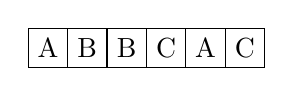
\begin{tikzpicture}[scale=1]
\draw (0,0.0) +(-.25,-.25) rectangle ++(.25,.25);
\draw (0,0.0) node{A};
\draw (0.5,0) +(-.25,-.25) rectangle ++(.25,.25);
\draw (0.5,0) node{B};
\draw (1.0,0) +(-.25,-.25) rectangle ++(.25,.25);
\draw (1.0,0) node{B};
\draw (1.5,0) +(-.25,-.25) rectangle ++(.25,.25);
\draw (1.5,0) node{C};
\draw (2.0,0) +(-.25,-.25) rectangle ++(.25,.25);
\draw (2.0,0) node{A};
\draw (2.5,0) +(-.25,-.25) rectangle ++(.25,.25);
\draw (2.5,0) node{C};
\end{tikzpicture}
\caption{Viewing an airplane as a a line of passengers.}
\end{figure}

In order to make all passengers happy in the smallest number of swaps, we first exchange seats 2 and 5 (which keeps the total number of happy families constant):

\begin{figure}[H]
\centering
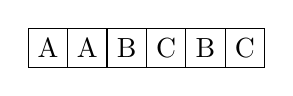
\begin{tikzpicture}[scale=1]
\draw (0,0.0) +(-.25,-.25) rectangle ++(.25,.25);
\draw (0,0.0) node{A};
\draw (0.5,0) +(-.25,-.25) rectangle ++(.25,.25);
\draw (0.5,0) node{A};
\draw (1.0,0) +(-.25,-.25) rectangle ++(.25,.25);
\draw (1.0,0) node{B};
\draw (1.5,0) +(-.25,-.25) rectangle ++(.25,.25);
\draw (1.5,0) node{C};
\draw (2.0,0) +(-.25,-.25) rectangle ++(.25,.25);
\draw (2.0,0) node{B};
\draw (2.5,0) +(-.25,-.25) rectangle ++(.25,.25);
\draw (2.5,0) node{C};
\end{tikzpicture}
\end{figure}

Then we exchange the passengers in seats 3 and 6:

\begin{figure}[H]
\centering
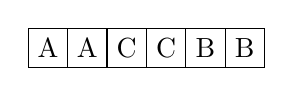
\begin{tikzpicture}[scale=1]
\draw (0,0.0) +(-.25,-.25) rectangle ++(.25,.25);
\draw (0,0.0) node{A};
\draw (0.5,0) +(-.25,-.25) rectangle ++(.25,.25);
\draw (0.5,0) node{A};
\draw (1.0,0) +(-.25,-.25) rectangle ++(.25,.25);
\draw (1.0,0) node{C};
\draw (1.5,0) +(-.25,-.25) rectangle ++(.25,.25);
\draw (1.5,0) node{C};
\draw (2.0,0) +(-.25,-.25) rectangle ++(.25,.25);
\draw (2.0,0) node{B};
\draw (2.5,0) +(-.25,-.25) rectangle ++(.25,.25);
\draw (2.5,0) node{B};
\end{tikzpicture}
\end{figure}

This second swap made 2 families happy with a single swap, and now all families are seated together. Please note that the family blocks are not in alphbetical order, and that any arrangement where all family membes are seated adjacent to each other is optimal.  

Also note that while this required only 2 swaps (the lowest possible for this input) that both swaps involved member of the ``B'' family.  Its possible to generate a pathological case where every swap involves the same passenger yet still minimizes the total number of swaps.  While this does not accurately reflect how grumpy this would make a passenger on our plane, our current model only cares about total number of swaps, future work will limit the maximum number of times a single passenger will have to swap.

\subsection{Limited Family Size Simplification}

While the general case allows passengers to fly together in arbitrarially large, heterogeneous groups, finding the optimal number of swaps in that case is NP-complete (see section \ref{sec:hardness}).  Because of this, we simplify the number of people who can belong to a family in two ways: either we limit the maximum family size in a heterogeneous assortment of families, or we demand all families be the same size.  

\section{Hardness} \label{sec:hardness}

For any case of the known NP-complete problem, 3-partition, there exists an initial passenger location assignment and family size combination where finding the minimum number of swaps possible would mean solving the 3-partition problem.  The reduction follows.

The 3-partition problem is defined as: Given a set of $n = 3m$ integers $x_i$, is there a grouping of the $x_i$ into $m$ disjoint triplets so that the sum of each triplet is the same number $k$?

For any 3-partition instance, we can design the seating arrangement as follows.  There are $m$ blocking families, $B_1, B_2... B_m$ all with the very large number of family members, $M_b > mk$.  For each $x_i$ there is a single family with $x_i$ family members, call these families $f_i$.  Finally there is a single huge family, the Seatwarmers, of size $\sum_i x_i = mk$, that we label $S$.

Our initial seating arrangement is to sit exactly $k$ seatwarmers in the first seats, followed by every member of $B_1$, then alternate between placing a block of $k$ seatwarmers and family $B_i$ until we seat $B_m$ and all $mk$ seatwarmers.  After this we seat all remaining passengers in perfectly rifled order, i.e. $f_1 f_2 f_3 f_1 f_2 f_3 \hdots$.  We sketch this arrangement below (with k = 4, M=2):

\begin{figure}[H]
\centering
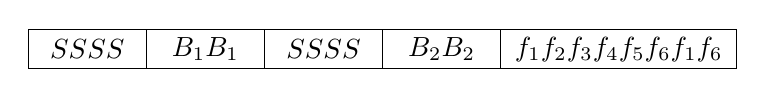
\begin{tikzpicture}[scale=1]
\draw (0,0.0) +(-.75,-.25) rectangle ++(.75,.25);
\draw (0,0.0) node{$SSSS$};
\draw (1.5,0) +(-.75,-.25) rectangle ++(.75,.25);
\draw (1.5,0) node{$B_1 \hdots B_1$};
\draw (3,0) +(-.75,-.25) rectangle ++(.75,.25);
\draw (3,0) node{$SSSS$};
\draw (4.5,0) +(-.75,-.25) rectangle ++(.75,.25);
\draw (4.5,0) node{$B_2 \hdots B_2$};
\draw (6.75,0) +(-1.5,-.25) rectangle ++(1.5,.25);
\draw (6.75,0) node{$f_1 f_2 f_3 f_4 f_5 f_6 f_1 f_6$};
\end{tikzpicture}
\end{figure}
\FloatBarrier

If this problem has a 3 partition, then in exactly $mk$ swaps we can make every family happy by swapping all of the seatwarmers in to the back of the plane, leaving the blocking families in place and in between each set of blocking families putting exactly 3 full $f_i$ families.  

Our toy instance's optimal seating arrangement is:

\begin{figure}[H]
\centering
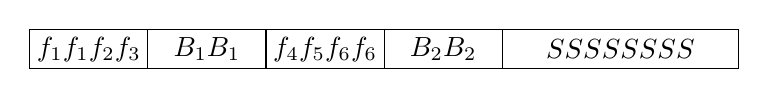
\begin{tikzpicture}[scale=1]
\draw (0,0.0) +(-.75,-.25) rectangle ++(.75,.25);
\draw (0,0.0) node{$f_1 f_1 f_2 f_3$};
\draw (1.5,0) +(-.75,-.25) rectangle ++(.75,.25);
\draw (1.5,0) node{$B_1 \hdots B_1$};
\draw (3,0) +(-.75,-.25) rectangle ++(.75,.25);
\draw (3,0) node{$f_4 f_5 f_6 f_6$};
\draw (4.5,0) +(-.75,-.25) rectangle ++(.75,.25);
\draw (4.5,0) node{$B_2 \hdots B_2$};
\draw (6.75,0) +(-1.5,-.25) rectangle ++(1.5,.25);
\draw (6.75,0)node{$SSSSSSSS$};
\end{tikzpicture}
\end{figure}

\begin{lem}
$mk$ is the minimum number of required swaps $\forall m > 2$
\end{lem}

\begin{proof}
If the seatwarmers all sit together in the back of the plane, it requires one swap per seatwarmer to get back there, or exactly $mk$ swaps.  

By contradiction, assume the seatwarmers don't sit in the final block in the back of the plane.  This means some members of a blocking family $B_i$ have to move.  As long as $M_B > mk$, there are more blocking members in any family than there are seatwarmers, so at most $k$ seatwarmers don't have to change their seat.  Getting the rest to sit in this unmoving block will require $(m-1)k$ swaps.

However, there are now $(m-1)k$ blocking members sitting in the wrong seats.  Since any exchange either puts 0,1 or 2 people in their optimal location, it takes a minimum of $\frac{(m-1)k}{2}$ exchanges to make these blocking members happy.  So long as $\frac{3(m-1)}{2} >= m$ or $m>=3$, this is no better than the $mk$ swaps we achieved using the initial method.
\end{proof}


\section{Solved Cases}

\subsection{Family size of exactly 2}

\noindent
Let us assume that we only have couples on-board, maybe a plane full of honeymooners headed to a post-nuptial resort. For this case, the following sweeping-line algorithm was proposed:

\begin{algorithm}
\caption{ \texttt{Sweep algorithm for families of size two} }
\label{alg:twoSweep}
  \begin{algorithmic}
\While{ $i \leq n-2$ }
  \State Read a pair ($i$, $i+1$) 
  \If{ $couple(i) \neq couple(i+1)$}
   \State let $j = i+2$
   \While{ $couple(j) \ne couple(i)$}
      $j = j + 1$
   \EndWhile
   \State Swap (j, i+1)
  \EndIf
\EndWhile
\caption{ \texttt{Sweep algorithm for families of size two} }
\end{algorithmic}
\end{algorithm}
\FloatBarrier

\begin{thm} \label{thm:sweepCorrectness}
There exists an optimal set of single passenger exchanges where the leftmost position of passengers involved in each exchange is non-decreasing.
\end{thm}


If we imagine a solution to this problem as an ordered pair of seat numbers to be exchanged, $(i_1,j_1), (i_2,j_2)...$ then the following observation can be made. 

\begin{lem} \label{lem:swapRules} 
We can change the order of exchanges using the three rules (with $a,b,c,d$ being unique seat numbers) without changing the final permutation achieved by performing these swaps.

\begin{eqnarray*}
(a,b) (c,d) \rightarrow (c,d) (a,b) \\
(a,b) (a,c) \rightarrow (a,c) (c,b) \\
(a,b) (b,c) \rightarrow (b,c) (a,c) \\
(a,b) (c,a) \rightarrow (c,a) (c,b) \\
\end{eqnarray*}
\end{lem}

\begin{proof}
Assume an odered pair of exchanges has the two exchanges $(a,b) (c,d)$ occurring in sequence. If either $a=b$ or $c=d$, that exchange does nothing and isn't optimal.  By the commutativity of a single exchange, we can insist that $a<b$ and $c<d$.  If $a=b$ and $c=d$, then these two exchanges do nothing and are also not optimal.  The final two cases are that one element of $(a,b)$ is equal to another from $(c,d)$ or that all 4 elements are unique.

When all four elements are unique, performing the first exchange does not change the initial position of either passenger in the second exchange and thus the two exchanges can be completed in any order and preserve exactly the final permutation.

When there is a shared seat being exchanged in both, as in $(a,b) (b,c)$ performing exchange 2 first would change the inhabitant of the repeated seat ($b$) in exchange 1.  Since the previous inhabitant of this seat is now located in the non-shared seat location from the exchange 2, if we want to perform exchange 2 first then we must change exchange 1's shared element ($b$) to the non-shared element of exchange 2 ($c$) in order to perserve the final permuation.
\end{proof}

Proving theorem \ref{thm:sweepCorrectness} is now trivial.

\begin{proof}
If we are given an optimal set of exchanges that are in non-decreasing order of leftmost passenger, we can transform it into a set of exchanges using the same number of swaps that is in non-decreasing order by combining a bubble sort and lemma \ref{lem:swapRules}.

First, we insist that all exchanges be listed with their lowest index first.  Ten we note that in all swaps where an exchange is modified by the rules of lemma \ref{lem:swapRules}, even after making the modifications, the modified exchange will never have a first index smaller than that of the exchange that we just swapped it for.

Finally, starting at exchanges $n-1$ and $n$, we swap the exchanges if the first index of exchange $n$ is lower than that of the exchange $n-1$, and then move on to comparing exchanges $n-1$ and $n-2$.  After one pass, the exchange with lowest left passenger would be our first element. After $n$ passes, the list will be sorted.
\end{proof}

We have only proven that there exists a left to right sweep algorithm that will allow us to seat all couples together, not that our specific sweep algorithm is optimal.  To bridge this gap, we need to make the following observations.

First, because the plane is full of couples, each pair of aligned adjacent seats (where aligned means the first is an odd numbered seat and the second an even numbered seat) will hold a matched couple in the final arrangement.  Any pair of seats in the initial seating arrangement that is not occupied by a matched couple will require at least one exchange to remedy that.

Second, any sweep algorithm will start with the leftmost aligned pair of seats containing a mismatched couple and swap one of those two inhabitants with another passenger in the plane.  Once we prove below that all exchange choices leave the plane in a state that requires the same number of swaps, we can claim that our sweep algorithm is optimal.

\begin{lem} \label{lem:identicalToRelabel}
All exchanges that make one couple happy are equivalent up to a relabeling.
\end{lem}

\begin{proof}
If the first two passengers are parts of the $A$ and $B$ couple, their partners are in one of two configurations (where we only show seats occupied by one member of the $A$ or $B$ couple):
\begin{figure}[H]
\centering
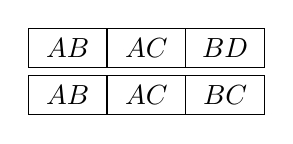
\begin{tikzpicture}[scale=1]
\draw (0,0.0) +(-.5,-.25) rectangle ++(.5,.25);
\draw (0,0.0) node{$A B$};x
\draw (1.0,0) +(-.5,-.25) rectangle ++(.5,.25);
\draw (1.0,0) node{$A C$};
\draw (2.0,0) +(-.5,-.25) rectangle ++(.5,.25);
\draw (2.0,0) node{$B C$};
\draw (0.0,.60) +(-.5,-.25) rectangle ++(.5,.25);
\draw (0.0,.60) node{$A B$};
\draw (1.0,.60) +(-.5,-.25) rectangle ++(.5,.25);
\draw (1.0,.60) node{$A C$};
\draw (2.0,.60) +(-.5,-.25) rectangle ++(.5,.25);
\draw (2.0,.60) node{$B D$};
\end{tikzpicture}
\end{figure}
For the first configuration, we can swap $A$ to be with its partner in either the first or second block:
\begin{figure}[H]
\centering
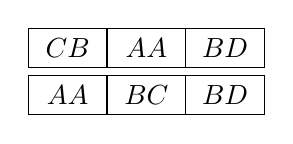
\begin{tikzpicture}[scale=1]
\draw (0,0.0) +(-.5,-.25) rectangle ++(.5,.25);
\draw (0,0.0) node{$A A$};
\draw (1.0,0) +(-.5,-.25) rectangle ++(.5,.25);
\draw (1.0,0) node{$B C$};
\draw (2.0,0) +(-.5,-.25) rectangle ++(.5,.25);
\draw (2.0,0) node{$B D$};
\draw (0.0,.60) +(-.5,-.25) rectangle ++(.5,.25);
\draw (0.0,.60) node{$C B$};
\draw (1.0,.60) +(-.5,-.25) rectangle ++(.5,.25);
\draw (1.0,.60) node{$A A$};
\draw (2.0,.60) +(-.5,-.25) rectangle ++(.5,.25);
\draw (2.0,.60) node{$B D$};
\end{tikzpicture}
\end{figure}
Other than changing which pair of seats are occupied, we have a happy couple $A$ and two pairs of unhappy patrons, $BC$ and $BD$.  These configurations require the exact same number of swaps to rectify.

If we instead swapped $B$, we'd get two configurations also:
\begin{figure}[H]
\centering
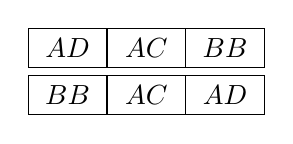
\begin{tikzpicture}[scale=1]
\draw (0,0.0) +(-.5,-.25) rectangle ++(.5,.25);
\draw (0,0.0) node{$B B$};
\draw (1.0,0) +(-.5,-.25) rectangle ++(.5,.25);
\draw (1.0,0) node{$A C$};
\draw (2.0,0) +(-.5,-.25) rectangle ++(.5,.25);
\draw (2.0,0) node{$A D$};
\draw (0.0,.60) +(-.5,-.25) rectangle ++(.5,.25);
\draw (0.0,.60) node{$A D$};
\draw (1.0,.60) +(-.5,-.25) rectangle ++(.5,.25);
\draw (1.0,.60) node{$A C$};
\draw (2.0,.60) +(-.5,-.25) rectangle ++(.5,.25);
\draw (2.0,.60) node{$B B$};
\end{tikzpicture}
\end{figure}

These cases are, exactly like the $A$ swapping cases, equivalent in terms of how many swaps would be required to finish pairing the rest of the plane.  The second possible initial case (where $A$ and $B$ are both seated next to family $C$, yields similarly equivalent situations after an exchange for $A$:
\begin{figure}[H]
\centering
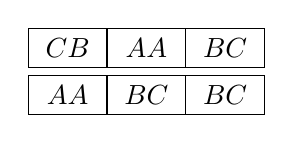
\begin{tikzpicture}[scale=1]
\draw (0,0.0) +(-.5,-.25) rectangle ++(.5,.25);
\draw (0,0.0) node{$A A$};
\draw (1.0,0) +(-.5,-.25) rectangle ++(.5,.25);
\draw (1.0,0) node{$B C$};
\draw (2.0,0) +(-.5,-.25) rectangle ++(.5,.25);
\draw (2.0,0) node{$B C$};
\draw (0.0,.60) +(-.5,-.25) rectangle ++(.5,.25);
\draw (0.0,.60) node{$C B$};
\draw (1.0,.60) +(-.5,-.25) rectangle ++(.5,.25);
\draw (1.0,.60) node{$A A$};
\draw (2.0,.60) +(-.5,-.25) rectangle ++(.5,.25);
\draw (2.0,.60) node{$B C$};
\end{tikzpicture}
\end{figure}

And $B$

\begin{figure}[H]
\centering
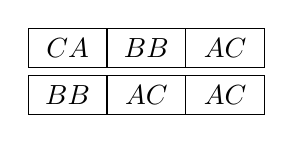
\begin{tikzpicture}[scale=1]
\draw (0,0.0) +(-.5,-.25) rectangle ++(.5,.25);
\draw (0,0.0) node{$B B$};
\draw (1.0,0) +(-.5,-.25) rectangle ++(.5,.25);
\draw (1.0,0) node{$A C$};
\draw (2.0,0) +(-.5,-.25) rectangle ++(.5,.25);
\draw (2.0,0) node{$A C$};
\draw (0.0,.60) +(-.5,-.25) rectangle ++(.5,.25);
\draw (0.0,.60) node{$C A$};
\draw (1.0,.60) +(-.5,-.25) rectangle ++(.5,.25);
\draw (1.0,.60) node{$B B$};
\draw (2.0,.60) +(-.5,-.25) rectangle ++(.5,.25);
\draw (2.0,.60) node{$A C$};
\end{tikzpicture}
\end{figure}

In all cases, exchanging either $A$ or $B$ first left us with conifgurations that were identical up to relabeling $A$ and $B$.  Further, swapping $A$ or $B$ out of the first pair into the seat beside its partner left us with identical configurations up to a reordering of seats.
\end{proof}

Since all sweep algorithms that make at least one couple happy with every exchange are equivalent, and there exists an optimal sweep algorithm that does exactly that, we have proven that our sweep alorithm finds the lowest number of required exchanges.

\section{Mixed families -- couples and singletons}

Let us now consider the case where we have a mixture of couples and singletons, where we want to seat all of the couples together. We assume that singletons are always happy, regardless of whom they sit next to.

\subsection{Phase One, determining structure:} 

We first observe that the worst case scenario for performing exchanges is when we have a situation like:

\begin{equation*}
eAABBCCDDe
\end{equation*}

This requires 4 swaps, or one swap per couple between the two unhappy members of the $e$ pair.  In terms of defining structure beforehand, this was an example of the following situation (where solid boxes will be occupied by a couple, and dotted by singletons):

\begin{figure}[H]
\centering
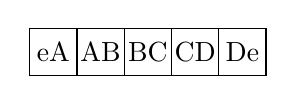
\begin{tikzpicture}[scale=1]
\draw (0.0,0) +(-.3,-.3) rectangle ++(.3,.3);
\draw (0.0,0) node{eA};
\draw (0.6,0) +(-.3,-.3) rectangle ++(.3,.3);
\draw (0.6,0) node{AB};
\draw (1.2,0) +(-.3,-.3) rectangle ++(.3,.3);
\draw (1.2,0) node{BC};
\draw (1.8,0) +(-.3,-.3) rectangle ++(.3,.3);
\draw (1.8,0) node{CD};
\draw (2.4,0) +(-.3,-.3) rectangle ++(.3,.3);
\draw (2.4,0) node{De};
\end{tikzpicture}
\end{figure}

With this assignment, we can clearly see that all passengers are seated in an incorrect seat to start. If instead the two $e$ passengers were singletons, then the following structural assignment would have allowed us to keep all passengers in their starting seats and require zero swaps.

\begin{figure}[H]
\centering
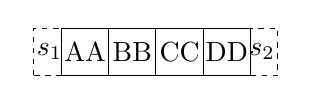
\begin{tikzpicture}[scale=1]
\draw[dash pattern= on 2pt off 2pt] (0,0) +(-.2,-.3) rectangle ++(.15,.3);
\draw (0.0,0) node{$s_1$};
\draw (0.45,0) +(-.3,-.3) rectangle ++(.3,.3);
\draw (0.45,0) node{AA};
\draw (1.05,0) +(-.3,-.3) rectangle ++(.3,.3);
\draw (1.05,0) node{BB};
\draw (1.65,0) +(-.3,-.3) rectangle ++(.3,.3);
\draw (1.65,0) node{CC};
\draw (2.25,0) +(-.3,-.3) rectangle ++(.3,.3);
\draw (2.25,0) node{DD};
\draw[dash pattern= on 2pt off 2pt] (2.7,0) +(-.15,-.3) rectangle ++(.2,.3);
\draw (2.7,0) node{$s_2$};
\end{tikzpicture}
\end{figure}

To properly assign a structure to a seating arangement for singletons and couples that minimizes swaps, we generalize the above bad example.  Sets of paired individuals already seating by their partners are called {\it blocks}.  Our bad example had $AABBCCDD$ all starting in good places, and thus we had a block of $N = 4$ couples.  Our block was out of alignment with our first seating type assignment and would require $N$ swaps to satisfy all seating requirements.  On the other hand, the block was in perfect alignment with the second seating type assignment and required no swaps to be seated.

\begin{figure}[H]
\centering
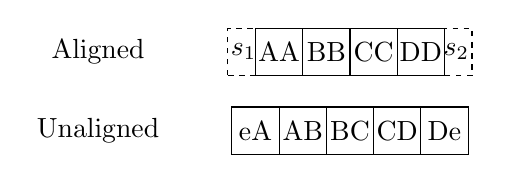
\begin{tikzpicture}[scale=1]
\draw (-2,1) node{Aligned};
\draw[dash pattern= on 2pt off 2pt] (-0.15,1) +(-.2,-.3) rectangle ++(.15,.3);
\draw (-0.15,1) node{$s_1$};
\draw (0.3,1) +(-.3,-.3) rectangle ++(.3,.3);
\draw (0.3,1) node{AA};
\draw (0.9,1) +(-.3,-.3) rectangle ++(.3,.3);
\draw (0.9,1) node{BB};
\draw (1.5,1) +(-.3,-.3) rectangle ++(.3,.3);
\draw (1.5,1) node{CC};
\draw (2.1,1) +(-.3,-.3) rectangle ++(.3,.3);
\draw (2.1,1) node{DD};
\draw[dash pattern= on 2pt off 2pt] (2.55,1) +(-.15,-.3) rectangle ++(.2,.3);
\draw (2.55,1) node{$s_2$};

\draw (-2,0) node{Unaligned};
\draw (0.0,0) +(-.3,-.3) rectangle ++(.3,.3);
\draw (0.0,0) node{eA};
\draw (0.6,0) +(-.3,-.3) rectangle ++(.3,.3);
\draw (0.6,0) node{AB};
\draw (1.2,0) +(-.3,-.3) rectangle ++(.3,.3);
\draw (1.2,0) node{BC};
\draw (1.8,0) +(-.3,-.3) rectangle ++(.3,.3);
\draw (1.8,0) node{CD};
\draw (2.4,0) +(-.3,-.3) rectangle ++(.3,.3);
\draw (2.4,0) node{De};
\end{tikzpicture}
\end{figure}

To fully represent a starting seating arrangement, we must note which passengers are not in blocks, contigious seats thus occupied will be called gaps.  While all blocks will be of even length (because they're comprised of couples), gaps can be of even or odd length.  I will refer to the parity of a gap as odd or even depending on whether the number of elements in it are odd or even.

\begin{lem} \label{lemma:ParityOnly}
For each starting block of size $N_i$, the optimal structural assignment will have a contiguous block of $N_i$ coupled seats. These can either be at the starting location or offset from that position by 1.
\end{lem}

\begin{proof}[Proof that contiguous blocks remainin in place.]
By contradiction.  Let's suppose that the first (left) $k$ couples are declared to be aligned improperly with seats asigned to couples, and the remaining $N-k$ to be aligned properly.  In order for this to occur, there had to be a singleton seat at the transition from aligned to unaligned.  

In order for this structural assignment to be optimal, there can't be a place to put this singleton that would require fewer swaps than the middle of this block.  However, placing it to the left of the $k$ unaligned couples would allow them to all be properly aligned, and reduce the number of swaps required by $k$.
\end{proof}

This in hand, we are going to ask how many existing blocks are going to have to be declared unaligned in order to globally minimize the number of swaps we perform. When a block is declared unaligned, we mean that instead of saying its first and second passengers (who are presupposed to be a couple due to this being a block) are in a single pair of couple designated seats, that instead they are siting in two different designated paired seats.  i.e.


We need another lemma before we can get an algorithm out of these observations.

\begin{lem} \label{lem:oddGapsNeedSingletons}
To satisfy all couples in an odd parity gap without disturbing its neighboring blocks, an odd number of singleton seats will be assigned to the gap.
\end{lem}

\begin{proof}
All seats not assigned to a singletons are assigned in pairs to couples.  All assigned couples take up an even number of seats leaving an odd number of seats to fill with singletons.
\end{proof}

\begin{cor}
All odd gaps require at least one singleton seat to be assigned to it.
\end{cor}

\begin{cor}
Any structural assignment with more odd parity gaps than singleton passengers will require that some blocks move.
\end{cor}

So which blocks move?  With $O$ representing a gap of odd parity, $E$ a gap of even parity, and $B$ being a block, the following situations exhaustively describe gap-block borders:

\begin{align*}
O B O \\
E B O \\
O B E \\
E B E \\
O B_1 E B_2 E B_3 \hdots B_k O \\
\end{align*}

In the first situation, if we declare the block unaligned and then perform the $N$ couple swaps to make it a block again, we wind up with $E B E$ and two fewer odd parity gaps.  

If we declare the block unaligned in the second or third cases, and preform $N$ couple swaps to make it a block again, we wind up with $O B E $ and $E B O$ respectively but keep the number of odd parity gaps constant.  The third case would become $O B O$, generating two aditional odd parity gaps.

The final case would become $E B_1 E B_2 E \hdots B_k E$.  This would reduce the number of odd parity gaps by 2 and cost $\sum_{i=1}^k |B_i|$ swaps.  Please note that only shifts between adjacent odd parity gaps decrease the number of odd parity gaps that we have, that all such shifts decrease our number of odd parity gaps by 2 and that they all cost a number of swaps equal to the number of couples in the blocks between them all.

\begin{lem} \label{lem:shiftLeftRightIdentical}
Shifting a block surrounded by odd gaps either to the right or left makes both of its odd parity gap neighbors even, and are equivalent in terms of total swaps left to pair all couples.
\end{lem}

\begin{proof}
The gap reduction part was argued above, so we need only prove equivalence.  A block bordered by two odd gaps has two neighbor passengers, $x$ and $y$.  After moving the block one to the left, we will shift passenger $x$ to the right side of the block, immediately before passenger $y$.  If $x$ and $y$ match, they increase the size of the block, if they don't, we know that $y$ didn't match its right neighbor otherwise it would have been a part of a block rather than an odd gap.

If we move the block to the right, then passenger $y$ winds up one unit to the left of the block next to $x$ again. Since we know that $x$ wasn't partnered with its neighbor to the left, the only new passible partnership is, as before, $x$ and $y$.

Thus moving a block left or right are equivalent in terms of number of swaps left to complete all pairings.
\end{proof}

\subsection{Dynamic Program for Gap Assignment}

A simple dynamic program can answer the question: which blocks do we declare unaligned in the optimal seating structure?  

Diagramatically, we have:

\begin{figure}[H]
\centering
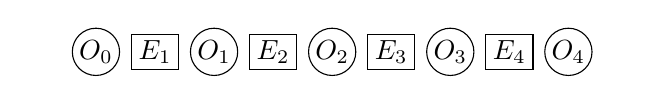
\begin{tikzpicture}[scale=.75]
\draw (0.5,0) node{$\hdots$};

\draw (1.8,.3) +(-.3,-.3) circle (.4);
\draw (1.5,0) node{$O_0$};

\foreach \x in {1, 2, 3, 4}
{
  \draw (0.5+2*\x,0) +(-.4,-.3) rectangle ++(.4,.3);
  \draw (0.5+2*\x,0) node{$E_\x$};
  \draw (2*\x+1.8,.3) +(-.3,-.3) circle (.4);
  \draw (2*\x+1.5,0) node{$O_\x$};
}
\draw (10.3,0) node{$\hdots$};
\end{tikzpicture}
\end{figure}

$E_i$, the block or $B_1EB_2E...B_k$ complex between odd gap $i-1$ and $i$ has $N_i$ paired couples.  We label the number of required swaps to fix parity $S(x,k)$ where $x$ is the index of the block we're moving and $k$ is the number of odd parity gaps we've closed.

Our recurrence relation is: 

\begin{equation*}
  S(x,k) = \min S(x-2, k-2) + N_{x}, S(x-1,k)
\end{equation*}

Memoizing this table takes the number of odd gaps times the number of gaps we have to close.  Since each odd gap lies between two blocks, the number of odd gaps is no more than $\frac13$ of our total number of seats.  We can't close more gaps than we have, so this simple algorithm is worst case quadratic in number of passengers.  

\subsection{Performing the Swap Sweep}

After the dynamic program is run, we perform the swaps it indicated.  This leaves us with a set of subproblems, the gaps between blocks (who will not move again).  Even gaps are easier to solve than odd gaps because their parity is already set, so we'll start with them.  While sweeping through a gap, we look at two elements at a time, seats $i$ and $i+1$.  With $s$ representing singletons, and all capital letters representing couple members, there are five distinct cases, each of which get treated differently.

\begin{itemize}
\item $AA$ 
Though it would seem that this shouldn't happen as gaps are filled with unpaired passengers, earlier steps in our sweep algorithm can leave these completed pairings in place.  When enountered, leave them there.
\item $AB$ 
The same arguments from Lemma \ref{lem:identicalToRelabel} hold here and swapping either $A$ or $B$ with its pair elsewhere in the plane leaves the passenger arrangement identical up to a relabeling.  When encountered, swap $B$ for the partner of $A$.
\item $As$
The same arguments from Lemma \ref{lem:identicalToRelabel} hold here with some slight modification. The relabeling would be calling 2 specific singletons $A$.  Since singletons have the potential to be left in place (saving swaps) swapping in the partner to $A$ will always be the optimal answer.  When encountered, exchange $s$ for the partner for $A$.
\item $sA$ 
This case is more complicated, as we can leave the singleton in place if we have 2 more singletons than we have odd parity gaps, and we have a complementary $Bs$ in this same gap.  When encountered, if we have 2 extra singletons in the budget, scan from right of this gap. If there is a matching $Bs$, leave both singletons in place and turn this gap into 2 new gaps: the one between these 2 singletons, and the gap between the right singleton and the next block.  Else, swap the $s$ for the matching $A$.
\item $ss$ 
Leave in place permanently if we have 2 more free singletons than odd parity gaps, temporarially if we are going to have to use these singletons.
\end{itemize}

By Lemma \ref{lem:identicalToRelabel}, and the observation that when an swap is identical up to a relabel, if the singletons are moved to an incomplete portion of the plane, they can never require more swaps than if we instead moved halves of couples.

\begin{lem} \label{lem:splitOddGaps}
Permanently leaving a singleton at an odd position in an odd length gap partitions it into 2 even length gaps that can be scanned using the above rules.
\end{lem}

Following this order, we have 2 types of odd length gaps left: those with singletons in even numbered seats (counting from their first seat) and those with no singletons.  Each of these gaps needs 1 singleton in an odd numbered seat to apply Lemma \ref{lem:splitOddGaps} and then scan using the even gap rules.  To scan odd gaps with singletons in them, we add in one rule:

\begin{itemize}
\item{$As$}
To save a single exchange, if the other $A$ is in an odd seat, exchange the $s$ for that $A$ and then use even scan rules on the 2 even gaps just created.  If the other $A$ is in an even seat, exchange this pair from $As$ to $sA$ and continue this gap as if it were even.
\end{itemize}

With only odd length gaps remaining that have no singletons in them, we need to swap in singletons that were left in their original seats using the $ss$ rule.  While scnaning these gaps, we use the simple rules:

\begin{itemize}
\item{$A_1 B$}
If $A_2$ is also in an odd seat, trade both $A_1$ and $A_2$ for a pair of singletons sitting next to each other in a completed gap. Then complete the 3 newly created even gaps using the even gap rules.
\item{$A_1-$}
When we reach the end of a gap without encountering the previous situation, trade both $A_1$ and $A_2$ for a pair of singletons sitting next to each other in a completed gap. Then scan the gap that previously contained $A_2$.
\end{itemize}

\subsection{Computer Simulations and Results}

In order to verify our hunch that the above algorithm was optimal, we coded up our algorithm in C++ and ran it on a PC. Each passenger was represented by a data structure: all passengers have a family name, a chair number, and know the family name of their left and right neighbors and the location of their partner.  Indices of seats occupied by singletons were stored in a single sorted array to allow range queries of singletons to occur in logarithmic time.

We sought to uncover the worst cases ecountered by our algorithm and devised the following simple test: starting from a completely content plane, we would select and exchange $k$ random passengers.  Because the optimal number of exchanges to return the plane to a completely content state must be no greater than $k$, we could compare the number of exchanges our algorithm found to $k$ in order to find the worst case performance ratio.  Any performance ratio less than 1 was discarded since this meant that the initial shuffling was simple enough that it could be undone in less than $k$ exchanges.

In order to find the high performance ratios, we allowed a genetic algorithm to search the space of shiffled seating arrangements.  For a plane of size $N$ with fixed $N_s \leq N$ singletons, the GA's genes first $N_s$ alleles were the indices of the singletons.  The next $2k$ indices were each interpreted as a pair of passenger positions to swap.  

The initial conifguration routine first sorted the list of singletons, then handled duplicate entries and having an odd number of seats between consecutive singletons. The vacant seats were occupied by content couples.  Finally the swapping portion of the genes were applied and passenger data structures were kept up to date with each swap.

It became almost immediately apparent that our algorithm was not optimal, as even modest sized problems ($N = 100, k = 10$) had worst case performance ratios above 1.6 after a few hundred generations.

\subsection{Win-Win Exchanges, Completed Couples and N-Chains}

Analysis of the genetic algorithm's worst case returns pointed us towards the following conclusion: we weren't handling win-win exchanges properly.  A win-win exchange is of the form:

\begin{figure}[H]
\centering
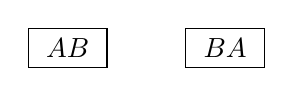
\begin{tikzpicture}[scale=1]
\draw (0,0.0) +(-.5,-.25) rectangle ++(.5,.25);
\draw (0,0.0) node{$A B$};x
\draw (2.0,0) +(-.5,-.25) rectangle ++(.5,.25);
\draw (2.0,0) node{$B A$};
\end{tikzpicture}
\end{figure}

We have two pairs of seats that can be satisfied completely with a single exchange. Since we cannot possibly make more than 2 couples happy with a single exchange, the optimal solution will contain as many of these as possible.  

\begin{lem} 
If a either of the seated couples in win-win exchanges are misaligned, it requires 2 swaps to make both pairs happy.
\end{lem}

\begin{proof}
Without loss of generality, we call the first, unaligned pair $A_1B_1$ and the second $A_2B_2$.  Since the first pair is unaligned, any exchange to pair it or its seatmate will necessarially not include $B_1$.  
\end{proof}

\begin{cor} \label{cor:winWinAsBlocks}
If a consecutive block of $N$ win-win pairs is misaligned, it requires $N$ more exchanges to satisfy all pairings than if they were all aligned.
\end{cor}

Win-win exchanges are 2 couples that can both be paired with a single exchange.  We would like to generalize this, calling win-win exchanges a 2-chain.  3-chains are three pairs that can all be satisfied with 2 exchanges like the example below:

\begin{figure}[H]
\centering
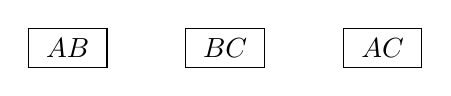
\begin{tikzpicture}[scale=1]
\draw (0,0.0) +(-.5,-.25) rectangle ++(.5,.25);
\draw (0,0.0) node{$A B$};x
\draw (2.0,0) +(-.5,-.25) rectangle ++(.5,.25);
\draw (2.0,0) node{$B C$};
\draw (4.0,0) +(-.5,-.25) rectangle ++(.5,.25);
\draw (4.0,0) node{$A C$};
\end{tikzpicture}
\end{figure}

This generalizes to $N$ chains, where chains are characterized by $N$ pairs that can all be satisfied with exactly $N-1$ swaps.

\subsection{Performance Ratio of Sweep Algorithm}

Our sweep algorithm ensures that we leave in place as many completed couples as possible. We do this because each completed couple we leave in place requires zero swaps, while setting them to be unaligned introduces new exchanges into our solution.  The ratio of unaligned exchanges to aligned exchanges is thus infinite, something to be avoided if we want a to bound the badness of a solution.

In its current incarnation, our algorithm ignores all $N$-chains.  Since each $N$-chain optimally requires $N-1$ swaps, failing to optimally align our couple seats will cost us at most $\frac{N}{N-1}$ times the optimal number of exchanges.  That is, our current algorithm is a 2 approximation.

\section{Conclusions}

We have introduced the novel problem of rearranging passengers on an airplane.  For even the special case of the airplane only having one row, we have shown in the general case of large families that this problem is NP complete.  The simple case of all passengers being in couples was solved optimally. For the more difficult case of all passengers being either alone or in couples, our algorithm was shown, first via simulations and then analytically, to be a 2 aproximation to optimal.

Our future work plans on analyzing heterogeneous family sizes larger than 2, and homogeneous small families as our hardness proof depended on arbitrarially large heteroeneous families. We would also like to analyze two dimensional planes with realistic seating arrangements, and families that nned not sit in one complete block, but where all family members has at least one familial neighbor.

Obviously, the optimization versions of all of these questions is also of interest.


\chapter{Genomic Interval Algorithm Analysis}{


\begin{centering}
\par{\large \bf Summary:}

\end{centering}

\par{Using a specific mathematical model, we treat DNA copy number analysis as an optimization problem. We devise a polynomaial time approximation scheme, two greedy heuristics and a binary programming model to solve the model exactly. These algorithms are analyzed for correctness and then their performance is tested using synthetic data.} 
}
\section{Introduction}

We have interpreted the DNA copy number analysis discussed in \cite{krasnitz2013target} as follows: given possibly overlapping ``defect'' intervals on a line, cover them with a set number of ``explanation'' intervals.  An explanation can only get credit for a defect if the explanation is a subset of said defect.  This is a special case of the maximum coverage problem, where our objective is to maximize the monotone submodular scoring function over a very structured set of subsets.  The hardness of this problem remains an open question.

\subsection{Prior Work} 

While the problem was formulated in relation to the CORE software product in \cite{krasnitz2013target}, the work done on related problems heavily influenced our algorithm development.  Our dynamic programming approach, as well as the definition of maximal explanations, started as an extension of the stabbing problem in \cite{katz2005orthogonal}. 

There is a graph formulation on which a maximum independent set would solve this problem. The heuristic approaches to maximal independent set in \cite{blelloch2012greedy} inspired those graph based approaches and lead directly to the counterexample to our LP relaxation constraint matrix being total unimodular. 

The $k$-OPT approach to maximum clique problem used in \cite{katayama2005effective} as well as previous exposure to the Lin-Kerrigan heuristic \cite{lin1973effective} motivated our own $k$-OPT algorithm.

\section{Description of the problem}

We imagine the genome as an interval graph. The set $D$ contains (possibly overlapping) intervals where damage has been observed.  We seek to find a set of $k$ explanations, $E$ that cover as much of $D$ as possible.

\begin{figure*}[ht!]
    \centering
        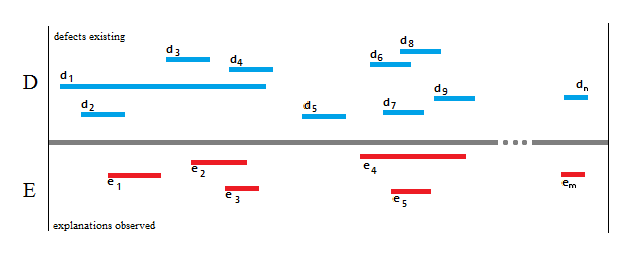
\includegraphics[width=0.99\textwidth]{baseline.png}
    \caption{a general description of the problem.}
\label{fig:genDesc1}
\end{figure*}

An explanation gets 'credit' for an area of overlap of a defect of which is it a proper subset. In figure~\ref{fig:genDesc1}, this means that $e_1$ may be allocated credit for explaining defect $d_1$, but not $d_2$.  The amount of credit for covering a defect is $\frac{ | e_i |}{|d_j|}$, i.e. the fraction of the defect covered by the explanation.
 
When two explanations $e_i,e_j$ overlap and both are a subset of a defect, they may be attributed at most $\frac{ | (e_i \cup e_j) |}{|d_k|}$. For example, in the above diagram, the intersection of $e_2$ and $e_3$ will be attributed as an explanation on $d_1$. They will be given no 'credit' for any explanation of $e_4$, because the segment is not a proper subset of $d_4.$

Goal : Given $k$ explanations, cover the maximum fraction of $D$.

\subsection{Definitions} 
\label{sec:definitions}

For the problem at hand, we have a set of defects $D = \{d_i\}$.  The endpoints of these defects are the integers $l_i, r_i$.  

We have a set of all relevant explanations $E = \{e_1, e_2, ... e_m\}$.  The number of explanations we can use is $k$.

The output explanation set from our algorithm is $A = \{S_1, S_2, ... S_k\}$.  Score($e_i | A$) is the improvement to our score from the explanation $e_i$ given that all of the explanations in $A$ are already in our solution.

The set $T = t_1, t_2, ... t_k$ is the optimal explanation set, i.e. the highest scoring set of $k$ explanations.  Score$(T) = $ OPT.

A {\it defect primitive} $d_{i,j}$ is the portion of defect $d_i$ between the consecutive endpoints $x_j$ and $x_{j+1}$, where $x_j$ and $x_{j+1}$ are the endpoints of any defect in the set.  As all maximal explanations start and end at these endpoint (from Lemma~\ref{lemma:Maximal}), defect primitives are atomic: either they are wholly explained or not explained at all.

\begin{figure}[H] \centering
  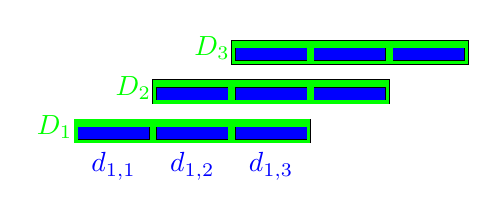
\begin{tikzpicture}[scale=1]

    \foreach \y in {1,2,3} {
      \draw (\y+1, \y/2) rectangle (\y+4, \y/2+.3);
      \fill[green] (\y+1, \y/2) rectangle (\y+4, \y/2+.3);
      \foreach \x in {1,2,3} {
        \draw (\x+\y+.05,\y/2 +.05) rectangle (\x+\y+.95,\y/2+.2);
        \fill[blue] (\x+\y+.05,\y/2 +.05) rectangle (\x+\y+.95,\y/2+.2);
      }
    }

    \foreach \x in {1,2,3} {
      \node[blue] at (1.5+\x,.5) [below] {$d_{1,\x}$};
    }
    
    
    \foreach \x in {1,2,3} {
      \node[green] at (\x+.75,.2+\x/2) {$D_\x$};
    }

  \end{tikzpicture} 
  \caption{{\color{green} Defects} and {\color{blue} defect primitives}.}
  \label{fig:defectPrimitives}
\end{figure}

A primitive's {\it depth} is the number of defects for which it is a subset.  

\subsection{Observation}

The following simplifying observation is useful:

\begin{lem} \label{lemma:Maximal}
Though any interval could be considered for membership in $E$, only ones that share endpoints with members of $D$ are interesting (i.e. candidates for inclusion in the maximal solution).  
\end{lem}

\begin{proof}
First off, explanations that are not proper subsets of any member of $D$ score nothing, so we ignore those.

By contradiction, the explanation $e = [a,b]$ is a proper subset of some number of defects, $G = \cap_i d_i$.  One or more of $a$ and $b$ are not endpoints of a defect.  The credit it gets is $\sum_i \frac{ (b-a) }{|d_i|} $, i.e. proportional to $(b-a)$.

Each $d_i \in G$ can be represented as $[l_i,r_i]$.  We construct the interval $[\max{l_i}, \min{r_i}]$.  Its credit is $\sum_i \frac{ (\min{r_i} - \max{l_i} ) }{|d_i|} $.  

Because $[a,b]$ is a subset of $G$, we know that $\forall_i a \geq l_i, b_i \leq r_i$.  Thus, $\min{r_i} - \max{l_i} \geq b-a$ where the inequality is only tight at $[a,b] = [\max{l_i}, \min{r_i}]$.  This contradicts the assumption that an interesting explanation doesn't share an endpoint with a defect.
\end{proof}

\section{Greedy Algorithm} \label{sec:greedy}

The obvious greedy algorithm would look at all possible explanations that could be placed, and place that explanation. This explanation would score certain portions of one or more defects.  The next step of the greedy algorithm would find the single explanation that scores the best in the presence of the existing solution.  

\begin{algorithm}
  \caption{ \texttt{greedyExplanationCover($D,k$)} }
  \label{alg:greedy}
  \begin{algorithmic}
    \State $M$ = set of maximal explanations
    \State $E = \emptyset$
    \While{ $|E| < k$ }
    \State $e_i = \argmax_{m\in M} S(D,m|E)$
    \State $E \leftarrow E \cup e_i$
    \EndWhile
    \State \Return $E$
  \end{algorithmic}
\end{algorithm}

\subsection{Automated Worst Case Generation}

In order to characterize the worst case performance ratio of \texttt{greedyExplanationCover($D$)}, we decided to first perform a black box analysis of its outputs.  Our methodology was simple: 

\begin{enumerate}
\item For fixed $k$, generate a defect set, $D$
\item Given $D$, compute the greedy explanation set $E$, and its score.
\item Compute optimum score and compare to the greedy score.
\end{enumerate}

To generate the defect endpoints, we randomly choose two integers per defect in the interval $[1,1000]$ and assign the lower (higher) to $l_i$ ($r_i$).  Because the underlying problem is on DNA with discrete base pair positions, integers were judged more appropriate than floating point positions.

Computing the optimum score is trivial for one special case of problems: the set of problems where $k$ = $|D|$.  In such cases, the optimal ouput set is just $D$ and the maximum score is $|D|$.  

\begin{tabular}{l|l}
k & $\frac{Greedy}{OPT}$ \\ \hline
 2 & .750001  \\
 3 & .779596  \\
 4 & .75361   \\
 5 & .800568  \\
 6 & .776081  \\
 7 & .806111  \\
12 & .931058  \\
36 & .995146  \\
\end{tabular}

Our results indicated that we should look at $\frac34$ as the performance ratio of the greedy algorithm.

\subsubsection{Worst Case Analysis}

Our computer simulations showed us scores for which we know cases exist on which greedy does poorly, and it also showed us the defect sets leading to said worst case behavior.  We performed case analysis for $k=2$ and $k=3$ to compare the computer's output with analytic results.

\paragraph{\textbf{$k=2$}} 

\begin{figure}[ht!] \centering
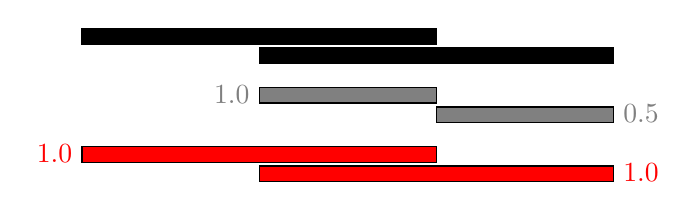
\begin{tikzpicture}[xscale=4.5,yscale=.5]

\fill[black] (0,4) rectangle (1,4.4);
\draw (0,4) rectangle (1,4.4);

\fill[black] (.5,3.5) rectangle (1.5,3.9);
\draw (.5,3.5) rectangle (1.5,3.9);


\fill[gray] (.5,2.5) rectangle (1,2.9);
\draw (.5,2.5) rectangle (1,2.9);
\node[gray] at (.5,3.2) [below left] {1.0};

%  \node[red] at (0,-.8) [above left] {$E_1$};

\fill[gray] (1,2) rectangle (1.5,2.4);
\draw (1,2) rectangle (1.5,2.4);
\node[gray] at (1.5,2.7) [below right] {0.5};

\fill[red] (0,1) rectangle (1,1.4);
\draw (0,1) rectangle (1,1.4);
\node[red] at (0,1.7) [below left] {1.0};

\fill[red] (.5,0.5) rectangle (1.5,0.9);
\draw (.5,0.5) rectangle (1.5,0.9);
\node[red] at (1.5,1.2) [below right] {1.0};

\end{tikzpicture} 
\caption{Worst case for $k=2$ Defects, \textcolor{gray}{Greedy solution} \textcolor{red}{Optimal solution}.  Numbers are scores of the explanation.}
\label{fig:k2}
\end{figure}

The first explanation placed has to score at least one, i.e. $S_1 \geq 1$, since it is the highest scoring explanation and covering either defect scores exactly one.  

For the second explanation, $S_2 \geq \frac{2 - S_1}{2}$.  This follows from a simple pidgeonhole argument: there are at most two defects with some regions uncovered.  The sum of those remaining scores is $2 - S_1$.  The higher scoring of those two defects has to yield at least half of this.  

Combining the two, we get $S_1 + S_2 \geq 1 + \frac{S_1}{2}$, this quantity is at least $\frac32$. 

The defect set in figure~\ref{fig:k2} would be scored $\frac32$ by the greedy algorithm, assuming it made the worst choice at the first step.

\paragraph{\textbf{$k=3$}} 

With 3 defects, we resort to case analysis.  A case will be defined by a table like:

\begin{tabular}{cccc}\hline
Round & Size & Score & Remainder \\ \hline
a & b & c & d \\
\end{tabular}

\begin{tabular}{l}
{\bf Round:} which explanation we're applying. \\
{\bf Size:} number of defects touched this round.  \\
{\bf Score:} score gained this round.  \\
{\bf Remainder:} total unexplained portions. \\
\end{tabular}

\begin{tabular}{cccc}\hline
Round & Size & Score & Remainder \\ \hline
1 & 3 & $\geq 1$ & 2 \\
2 & 1 & $\geq \frac23$ & $\frac43$ \\
3 & ? & $\geq \frac23$ & $\frac23$ \\
\end{tabular}

Where round 2's bound comes from the pigeonhole argument: with 3 total defects, and a score of 2 remaining, one yields at least $\frac23$.  Round 3 is also pigeonhole: in round 2 we completely covered one defect, the remainder of $\frac43$ is shared amongst 2 defects, thus one yields at least $\frac23$.

\begin{tabular}{cccc}\hline
Round & Size & Score & Remainder \\ \hline
1 & 3 & $S_1 \geq 1$ & 2 \\
2 & 2 & $S_2 + S_1 \geq 2$ & 1 \\
3 & ? & $\geq \frac13$ & $\frac23$ \\
\end{tabular}

In round one, we take fractions ${a,b,c}$ from the first, second and third defects.  WOLG, we say that in round 2, the two defects covered are the first and second for fractions $a_2 + b_2 = p$.  We know $a + b + p \leq a + b + c$ since $A \cap B$ wasn't covered in round one.  Thus $p \leq c$.  The remainders of each defect are also less than $p$: 

\begin{eqnarray*}
p \geq (1-a) & \rightarrow a \geq 1-p \\
p \geq (1-b) &\rightarrow b \geq 1-p \\
\end{eqnarray*}

Now we show how round one and two sum to a number greater than two:

\begin{eqnarray*}
S_1 = a+b+c &\geq (1-p) + (1-p) + c \\
S_1 &\geq 2 + c - 2p \\
S_2 &= p \\
S_1 + S_2 &\geq 2 + (c - p) \\
p \leq c &\rightarrow (c-p) \geq 0 \\
S_1 + S_2 &\geq 2 + (0) \\
\end{eqnarray*}

Round three is the standard pigeonhole argument.

\begin{tabular}{cccc}\hline
Round & Size & Score & Remainder \\ \hline
1 & 2 & $\geq 1$ & 2 \\
2 & ? & $\geq 1$ & 1 \\
3 & ? & $\geq \frac13$ & $\frac23$ \\
\end{tabular}

Round 2 has to be at least one since there was an untouched defect entering that round, and any maximum explanation has to score at least that much.  Then round three follows by pigeonhole.

\begin{tabular}{cccc}\hline
Round & Size & Score & Remainder \\ \hline
1 & 1 & $\geq 1$ & 2 \\
2 & ? & $\geq 1$ & 1 \\
3 & ? & $\geq \frac13$ & $\frac23$ \\
\end{tabular}

Exact same argument as above.

\paragraph{Concrete $k=3$ Example}

We've seen that the worst remainder we can achieve for 3 defects being covered with 3 explanations is $\frac23$.  This means greedy will score at least $\frac79$ of optimal.  Note: in figure~\ref{fig:k3}, only one of the three $\frac13$ gray explanations is chosen.

\begin{figure}[ht!] \centering
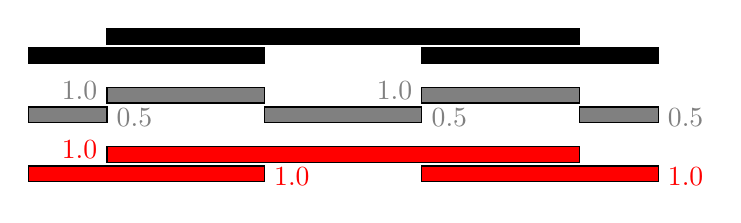
\begin{tikzpicture}[xscale=1,yscale=.5]

\fill[black] (1,4) rectangle (7,4.4);
\draw (1,4) rectangle (7,4.4);

\fill[black] (0,3.5) rectangle (3,3.9);
\draw (0,3.5) rectangle (3,3.9);

\fill[black] (5,3.5) rectangle (8,3.9);
\draw (5,3.5) rectangle (8,3.9);


\fill[gray] (1,2.5) rectangle (3,2.9);
\draw (1,2.5) rectangle (3,2.9);
\node[gray] at (1,3.3) [below left] {1.0};

\fill[gray] (5,2.5) rectangle (7,2.9);
\draw (5,2.5) rectangle (7,2.9);
\node[gray] at (5,3.3) [below left] {1.0};

% 1/3 row
\fill[gray] (0,2) rectangle (1,2.4);
\draw (0,2) rectangle (1,2.4);
\node[gray] at (1,2.6) [below right] {0.5};

\fill[gray] (3,2) rectangle (5,2.4);
\draw (3,2) rectangle (5,2.4);
\node[gray] at (5,2.6) [below right] {0.5};

\fill[gray] (7,2) rectangle (8,2.4);
\draw (7,2) rectangle (8,2.4);
\node[gray] at (8,2.6) [below right] {0.5};

\fill[red] (1,1) rectangle (7,1.4);
\draw (1,1) rectangle (7,1.4);
\node[red] at (1,1.8) [below left] {1.0};

\fill[red] (0,0.5) rectangle (3,0.9);
\draw (0,0.5) rectangle (3,0.9);
\node[red] at (3,1.1) [below right] {1.0};

\fill[red] (5,0.5) rectangle (8,0.9);
\draw (5,0.5) rectangle (8,0.9);
\node[red] at (8,1.1) [below right] {1.0};

\end{tikzpicture} 
\caption{Worst case for $k=3$ Defects, \textcolor{gray}{Greedy solution}, \textcolor{red}{Optimal solution}.  Numbers are scores of the explanation.}
\label{fig:k3}
\end{figure}

\subsubsection{Upper Performance Bound}

It is important to note that the example in figure \ref{fig:k2} can be extended for any even $N$. By placing $\frac{N}{2}$ non-overlapping copies along the number line we create an instance where the first $\frac{N}{2}$ explanations placed by the greedy algorithm score 1 while the next $\frac{N}{2}$ all score $\frac12$.  These sum to $\frac{3N}{4}$ which is clearly $\frac{3}{4}$ of the $N$ that an optimal soution would score.

\subsection{\texttt{MAXIMUM COVERAGE}}

\textit{AKA The $\frac{e-1}{e}$ Barrier}

For \texttt{MAXIMUM COVERAGE}, a related problem, the greedy algorithm is known to have an approximation ratio of  $(1-\frac{1}{e})$.  That is: 

\begin{thm} Given a set $P$ of sets $P_i$, the percentage of the total elements covered by the greedy algorithm can be as bad as $(1-\frac{1}{e})$ times OPT.
\end{thm}

\begin{proof} We define:

\begin{tabularx}{\linewidth}{l X}
{\bf OPT} & The most that can be covered by $k$ subsets. \\
{\bf $x_i$} & Amount covered by greedy in step $i$ \\
{\bf $y_i$} & Total covered by step $i$: $\sum_{j=0}^i x_i$ \\
{\bf $z_i$} & OPT$-y_i$ \\
\end{tabularx}

\begin{lem} \label{lem:MaxPidgeonhole}
For all $i$,  There exists subset where $x_{i+1} \geq \frac{z_i}{k}$.  
\end{lem}

\begin{proof}
Pidgeonhole.  OPT uses $k$ subsets in total.  The residual $z_i$ is no greater than the sum of score remaining in $A^*$, the subsets OPT uses. Since $ |A^*| = k$, one member of $A$ has at least $ \frac{z_i}{k}$ worth of score left. 
\end{proof}

\begin{eqnarray*}
x_{i+1} &\geq \frac{z_i}{k} \\
z_{i+1} &= z_i - x_{i+1} \\
z_{i+1} &\leq z_i - \frac{z_i}{k} = z_i( 1 - \frac{1}{k} ) \\
z_k    &\leq z_0 ( 1 - \frac{1}{k} )^k \\
\lim_{k \rightarrow \infty} ( 1 - \frac{1}{k} )^k &\leq ( 1 - \frac{1}{e}) \\
\lim_{k \rightarrow \infty} z_k &\leq z_0(1 -  \frac{1}{e}) 
\end{eqnarray*}

\end{proof}

\subsection{$k=4$ and Beyond}

After our case analysis and computer simulations, we were convinced that the set coverage greedy approximation factor of $1-\frac{1}{e}$ was overly pessimistic.  Our central contention was that the analysis leading to $1-\frac{1}{e}$ would require at each step for an explanation to hit every single defect.  This is not possible.

\begin{lem} \label{lemma: Number of primitives}
For a set of $n$ defects where all start and end points are unique, if there is one primitive of depth $n$, there is exactly 1, and there are exactly two primitives of each depth between 1 and $n-1$.
\end{lem}

\begin{proof}
This is most easily seen by scanning our endpoints from left to right.  As a left endpoint is reached, our depth increases by exactly one (since only 1 unique endpoint can be reached at once), as a right endpoint is reached, our depth decreases by exactly 1.

We start at depth 0, so to have a primitive of depth $n$, we must scan past exactly $n$ left endpoints and no right endpoints.  As there are only $n$ left endpoints in our defect set, we have exhausted our supply to get a single primitive of depth $n$.

Once we have scanned the first $n$ left endpoints, we passed through exactly $n$ primitives, each of unique depth.  As we continue, we will encounter all $n$ right endpoints.  Each of them will decrease our depth by 1 as we encounter it in our left to right scan, and thus mark the entrance into a new primitive of depths $n-1$, $n-2$, ... 1.  

With one primitive of each depth encountered to the left of our depth $n$ primitive, and another encountered right of our depth $n$ primitive, we have exactly 2 of each depth between 1 and $n-1$.
\end{proof}

Because we can arbitrarially break ties in starting and ending points by judiciously adding powers of $\epsilon$ to actual starting/ending positions, we can treat all defect sets as having unique starting and ending points.  Unfortunately, beyond this observation, we have no bound on how well greedy performs.

\subsection{1-OPT Improvement}

A natural refinement to the greedy algorithm is to improve its output by repeatedly asking whether any of its included explanations can be replaced with an unused explanation to improve the score.  This is known as \texttt{1-OPT} refinement.  

\begin{algorithm}
  \caption{ \texttt{1-OPTExplanationCover($D,k$)} }
  \label{alg:1-OPT}
  \begin{algorithmic}
    \State $E$ =  \texttt{greedyExplanationCover($D,k$)}
    \State haveExchanged = false
    \State $M$ = set of maximal explanations
    \Repeat
    \State haveExchanged = false
    \ForAll{$e_i \in E$}
    \State OldScore = $S(D,E)$
    \State $E' = E / e_i$
    \State $e = argmax_{m \in M} S(D,m|E')$
    \State NewScore = $S(D,e|E')$
    \If{OldScore $< $ NewScore }
    \State haveExchanged = true
    \State $E \leftarrow E' \cup e$
    \EndIf
    \EndFor
    \Until{haveExchanged = false}
    \State \Return $E$
  \end{algorithmic}
\end{algorithm}

In our results section, we will show how much of an imporvement \texttt{1-OPT} was over the greedy algorithm, but here we will show that it does not always lead to the correct answer.

\begin{figure}[h] \centering
    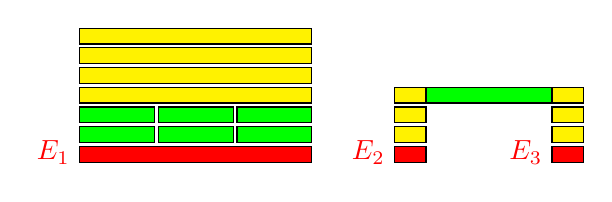
\begin{tikzpicture}[xscale=1,yscale=.5]

      % 6 small rectangles on the left in 2 rows of 3
      \foreach \x in {0,1,2} {
        \foreach \y in {0,1} {
          \fill[green] (0+\x,0+\y/2) rectangle (.95+\x,.4+\y/2);
          \draw (0+\x,0+\y/2) rectangle (.95+\x,.4+\y/2);
        }
      }
      
      % 4 Wide caps on those small rectangles
      \foreach \y in {0,1,2,3} {
        \fill[green] (0,1+\y/2) rectangle (2.95,1.4+\y/2);
        \draw (0,1+\y/2) rectangle (2.95,1.4+\y/2);
      }

      
      \foreach \y in {0,1} {
        \foreach \x in {4, 6} {
          \fill[green] (0+\x,0+\y/2) rectangle (.4+\x,.4+\y/2);
          \draw (0+\x,0+\y/2) rectangle (.4+\x,.4+\y/2);
        }
      }                  

      \fill[green] (4,1) rectangle (6.4,1.4);
      \draw (4,1) rectangle (6.4,1.4);

        \fill[red] (0,-.5) rectangle (2.95, -.1);
        \draw (0,-.5) rectangle (2.95, -.1);
        \node[red] at (0,-.8) [above left] {$E_1$};

        \foreach \y in {0,1,2,3} {
          \fill[yellow] (0,1+\y/2) rectangle (2.95,1.4+\y/2);
          \draw (0,1+\y/2) rectangle (2.95,1.4+\y/2);
        }

        \fill[red] (4,-.5) rectangle (4.4, -.1);
        \draw (4,-.5) rectangle (4.4, -.1);
        \node[red] at (4,-.8) [above left] {$E_2$};
        
        \fill[red] (6,-.5) rectangle (6.4, -.1);
        \draw (6,-.5) rectangle (6.4, -.1);
        \node[red] at (6,-.8) [above left] {$E_3$};

        
        \foreach \y in {0,1,2} {
          \foreach \x in {4, 6} {
            \fill[yellow] (0+\x,0+\y/2) rectangle (.4+\x,.4+\y/2);
            \draw (0+\x,0+\y/2) rectangle (.4+\x,.4+\y/2);
          }
        }                                               
     

    \end{tikzpicture}
    \caption{Initial Greedy Solution}
  \end{figure}          

The initial greedy solution's explanations are red.  It gets full credit for all yellow portions of explanations.  $E_1$ scores 4.  Both $E_2$ and $E_3$ score $2+\epsilon$.  Its score is $8 + 2\epsilon$.

\begin{figure}[h] \centering
  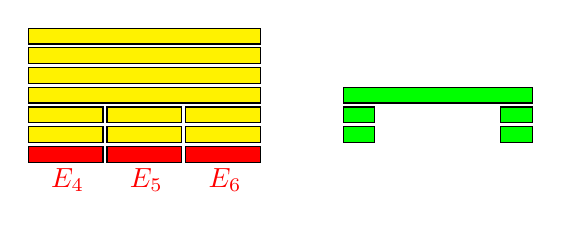
\begin{tikzpicture}[xscale=1,yscale=.5]

    % 6 small rectangles on the left in 2 rows of 3
    \foreach \x in {0,1,2} {
      \foreach \y in {0,1} {
        \fill[green] (0+\x,0+\y/2) rectangle (.95+\x,.4+\y/2);
        \draw (0+\x,0+\y/2) rectangle (.95+\x,.4+\y/2);
      }
    }
    
    % 4 Wide caps on those small rectangles
    \foreach \y in {0,1,2,3} {
      \draw (0,1+\y/2) rectangle (2.95,1.4+\y/2);
      \fill[green] (0,1+\y/2) rectangle (2.95,1.4+\y/2);
    }

    
    \foreach \y in {0,1} {
      \foreach \x in {4, 6} {
        \fill[green] (0+\x,0+\y/2) rectangle (.4+\x,.4+\y/2);
        \draw (0+\x,0+\y/2) rectangle (.4+\x,.4+\y/2);
      }
    }                  

    \fill[green] (4,1) rectangle (6.4,1.4);
    \draw (4,1) rectangle (6.4,1.4);

    \foreach \x in {4,5,6} {
      \fill[red] (-4+\x,-.5) rectangle (-3.05+\x,-.1);
      \draw (-4+\x,-.5) rectangle (-3.05+\x,-.1);
      \node[red] at (-3.5+\x,-1.5) [above] {$E_\x$};
    }

    \foreach \x in {0,1,2} {
      \foreach \y in {0,1} {
        \fill[yellow] (0+\x,0+\y/2) rectangle (.95+\x,.4+\y/2);
        \draw (0+\x,0+\y/2) rectangle (.95+\x,.4+\y/2);
      }
    }
    \foreach \y in {0,1,2,3} {
      \fill[yellow] (0,1+\y/2) rectangle (2.95,1.4+\y/2);
      \draw (0,1+\y/2) rectangle (2.95,1.4+\y/2);
    }
    
  \end{tikzpicture}
  \caption{Optimal Solution}
\end{figure}    

Each of $E_4, E_5, E_6$ score $3 \frac13$ for a total of 10.  

There is no single exchange from the greedy solution with any of the explanations in the optimal solution that improve the score.  Thus \texttt{1-OPT} is a useful refinement, but does not optimally solve the problem.

\texttt{$m$-OPT} refinement is the natural generalization when we ask if any set of $m$ explanations in the current solution can be replaced with another $m$ unused explanations to improve the score.  

\section{Dynamic Programming} \label{sec:DP}

A simple dynamic programming approach, where we score the $k+1$st defect and place all of them between points $a$ and $b$ such as $S(k+1,a,b) = \max_y S(k,a,y) + S(1,y,b)$ fails because the score, $ S(1,y,b)$, is dependent on the full state of which explanations are already placed.

Simply put, the barrier between solved and unsolved regions doesn't exist.

To get around this complication, we've proposed constant depth dynamic programming solutions.  Such a solution is characterized by the maximum number of explanations that can overlap at any one place in the solution.  A depth 1 dynamic programming solution would have no overlaps, and a depth 2 solution can have many regions where 2 explanations overlap, but none where 3 overlap.

\subsection{Depth 1 Dynamic Program} \label{sec:1DP}

A depth 1 dynamic program will find the set of explanations that cover any set of defects with the guarantee that no explanations will overlap.  The recurrence relation is simple: $S(k+1,0,x)$ = $\max_y S(k,0,y) + S(1,y,x)$.  The score we can achieve with $k+1$ explanations in the region $[0,x]$ is the max over intermediary points, $y$, of the score achieved before $y$ with $k$ explanations plus the score we can achieve to the right of $y$ with 1 explanation. The barrier between the completed subproblem and the unsolved region is the point $y$. We cannot place new explanations that start to the left of it.

The obvious question is: how well does this perform compared to an optimal solution which can overlap arbitrarially?

We will construct a non-overlapping solution, compare its value to OPT and then appeal to the correctness of a dynamic programming solution to claim that it will do this well or better.

To construct our solution, we will take OPT as an input.  The $k$ explanations of opt have associated with them $2k-1$ {\it explanation primitives}.  These are  {\it primitives} whose endpoints come from a set of explanations. There are $2k-1$ of them because no more than $2k$ unique points are required to describe $k$ defects.

Were we to use all of OPT's $2k-1$ explanation primitives, we would cover all defects that OPT covers.  If we select the $k$ highest scoring of these explanation primitives, we cover at least half of OPT's total credit. Unfortunately, this is worse than our greedy bound of $(1- \frac{1}{e})$.

\subsection{Depth $d$ Dynamic Program} \label{sec:dpFixedDepth}

For dynamic programs of depth $d \geq 2$, our state is slightly more complicated than it was for depth 1. We have $k$, the number of explanations used, $a$ the end of the solved region, $b$ the end of the active region and $S$, the {\it left} endpoints of the set of explanations that are active (there are up to $k$ of them) at point $b$ to form $DS(k,a,b,S)$.


\begin{figure}[ht!] \centering
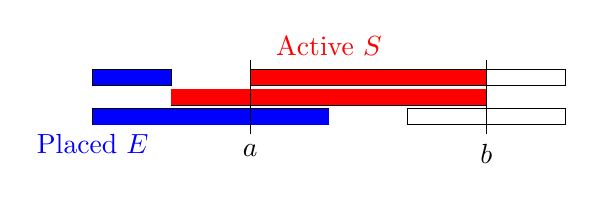
\begin{tikzpicture}[xscale=1,yscale=.25]

\draw (4,0) rectangle (6,0.8);

\draw (1,1) rectangle (5,1.8);
\fill[red] (1,1) rectangle (5,1.8);

\node[red] at (3,3) [above] {Active $S$};

\draw (2,2) rectangle (6,2.8);
\fill[red] (2,2) rectangle (5,2.8);

\draw (0,0) rectangle (3,0.8);
\fill[blue] (0,0) rectangle (3,0.8);

\draw (0,2) rectangle (1,2.8);
\fill[blue] (0,2) rectangle (1,2.8);

\node[blue] at (0,0) [below] {Placed $E$};


\draw (2,-.5) -- (2,3.3);
\node[black] at (2,-.5) [below] {$a$};

\draw (5,-.5) -- (5,3.3);
\node[black] at (5,-.5) [below] {$b$};

\end{tikzpicture} 
\caption{An illustration of a depth $d \geq 3$ DP in action.}
\label{fig:dpIllustration}
\end{figure}

\FloatBarrier

{\bf Running Time:} The memoization table can contain every legal state of the form $DS(k,a,b,S)$.  The first argument takes all values from 0 to $k$ inclusive.  The next two will only hold the values of endpoints, of which there are $2N$ of.  Each member of $S$ can be empty or hold the value of an endpoint, and there can be no more than $k$ members.  This gives us a total running time of: $O(kn^{2+k})$.

In order to build an optimal coverage that never exceeds a depth of $d$, the dynamic program sweeps.  Starting with $a$ and $b$ at the leftmost endpoint, we move them right respecting that $a \leq b$.  An explanation $(L,R)$ can become active iff $L\leq a$ and $R \geq b$ and $|S|<d$ for the current set $S$.

Each state $DS(k,a,b,S)$ has an associated explanation set $E$, the explanations that were placed earlier in the sweep and to attain the maximum current score for our state.  The following four transformations are sufficient to get from any starting state to any final state.

$ DS(k-1,a,b,S-e) \rightarrow DS(k,a,b,S)${\it A new explanation becomes active.} An explanation starting at $e$, where $e > x$ \hspace{4pt} $ \forall x \in S$, is added to our active list.

$ DS(k,a-1,a,S + (x,a)) \rightarrow DS(k,a,b,S)${\it An active explanation ends.}  Note the differing endpoints.  If we leave the ending explanation in the active region, it will be able to influence our current scoring region. Thus the active region moves to the right of the departing explanation.

$DS(k,a-1,b,S) \rightarrow DS(k, a, b, S )${\it Left boundary of active region contracts.} Since all explanations in $S$ start and end outside of $[a,b]$, this will not change the obtainable score.  It will, however, disqualify some candidates from joining the set $S$.

$DS(k,a,b-1,S) \rightarrow DS(k, a, b, S )${\it Right boundary of active region expands.} All active explanations in $S$ are treated as having $b$ as their right endpoint until they cease to be active.  Because of that, this movement can lead to explanations in $S$ to become non-scoring and is not always permitted.

\begin{lem} \label{lem:dpCorrect}
Using the rules outlined above, any legal explanation set could be reached.
\end{lem}

\begin{proof}
If we start any legal explanation set $E$ and convert it into the set of sorted endpoints $x_i$, the following sequence (in reverse) would find that set $E$.  

Start with $DS(k,x_k,x_k,\emptyset)$.  Use the ``active explanation ends'' rule  in reverse to get to the state: $DS(k,x_k,x_k,{x^L_k})$ where $x^L_k$ is the left endpoint of the explanation ending at $x_k$.

We can then use the left endpoint moving rule in reverse to get to $DS(k,x_{k-1},x_k,{x^L_k})$ and the right endpoint in reverse to get to $DS(k,x_{k-1},x_{k-1},{x^L_k})$.

If this is the right endpoint of an explantion, we will either use the ``active explanation ends'' as above.  If left, the ``new explanation becomes active'' rule in reverse will take us to the new predecessor state $DS(k-1,x_k,x_k,S_i \setminus{x^L_i} )$.

We would then continue shifting endpoints to $x_{i-1}$ and selecting the appropriate endpoint rule until we reach the leftmost extent of $E$.  With this construction, the members of $S_i$ at $x_i$ are those explanations stabbed by a line through that point.  Since the explanation set's depth is less than $d$, $|S_i|$ will also be less than $d$.  Thus these steps are all legal.
\end{proof}

\subsection{Quality of $d=2$ DP Solution}

Our result from section~\ref{sec:1DP} tells us that a depth 2 dynamic program will score no worse than the $\frac12$ of OPT that a depth 1 dynamic program will.  We can generalize that proof to find tighter bounds.

\begin{lem} \label{lem:2DP2/3}
Each of the $\frac{k}{2}$ subproblems formed by dividing an optimal solution after every fourth explanation primitive can have $65.5\%$ of its optimal score achieved with the use of 2 explanations.
\end{lem}

We prove this by exhaustively enumerating all possible 4 width subproblems, dismissing most of them with a counting argument and then exhaustively covering the remaining two with two explanations and finding the worst case behavior.

The border between any two explanation primitives occurs when an explanation is either ending or starting.  There are exactly three internal borders in any width four subproblem.  We will label classes of similar problems by the events they contain.  Using $1$ to represent a beginning, and $0$ an end, there are 8 naive classes of subproblems: $000, 001, 010 ... 111$.

Mirror image subproblems can be covered with mirror image explanations, and the mirror image of subproblem $abc$ is $\neg c \neg b \neg a$.  This leaves us with four distinct subproblem classes: $110, 101, 111, 011$. 

\subsubsection{Trivial Classes}

The first two classes, $110, 101$ can be drawn in multiple ways depending on which defect the $0$ terminates.  

\begin{figure}[h] \centering 
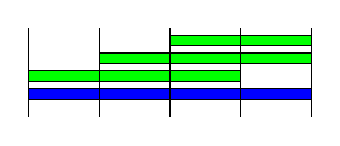
\begin{tikzpicture}[scale=.9]


\fill[blue] (0,.05) rectangle (4,.20);
\draw (0,.05) rectangle (4,.20);

\fill[green] (0,.30) rectangle (3,.45);
\draw (0,.30) rectangle (3,.45);

\foreach \x in {2,3} {
  \fill[green] (\x-1,\x/4 +.05) rectangle (4,\x/4+.20);
  \draw (\x-1,\x/4 +.05) rectangle (4,\x/4+.20);
}

\foreach \x in {0,1,2,3,4} {
    \draw (\x,-.2) -- (\x,1.05);
}


\end{tikzpicture} 
\caption{Class 110a}
\end{figure}

\begin{figure}[h] \centering 
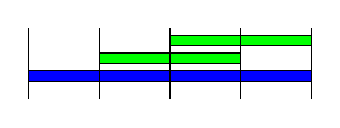
\begin{tikzpicture}[scale=.9]


\fill[blue] (0,.05) rectangle (4,.20);
\draw (0,.05) rectangle (4,.20);

\fill[green] (1,.30) rectangle (3,.45);
\draw (1,.30) rectangle (3,.45);

\fill[green] (2,.55) rectangle (4,.70);
\draw (2,.55) rectangle (4,.70);
 
\foreach \x in {0,1,2,3,4} {
    \draw (\x,-.2) -- (\x,.8);
}


\end{tikzpicture} 
\caption{Class 110b}
\end{figure}

\begin{figure}[h] \centering 
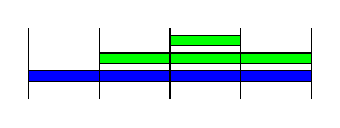
\begin{tikzpicture}[scale=.9]


\fill[blue] (0,.05) rectangle (4,.20);
\draw (0,.05) rectangle (4,.20);

\fill[green] (1,.30) rectangle (4,.45);
\draw (1,.30) rectangle (4,.45);

\fill[green] (2,.55) rectangle (3,.70);
\draw (2,.55) rectangle (3,.70);
 
\foreach \x in {0,1,2,3,4} {
    \draw (\x,-.2) -- (\x,.8);
}

\end{tikzpicture} 
\caption{Class 110c}
\end{figure}

All of the $110$ class members can be completely covered using as explanations the three green defects.  Since we are allowed to choose the two highest scoring of those three, clearly $\frac23$ of the optimal score is trivial for this class. The 101 class is smaller and similarly covered:

\begin{figure}[h] \centering 
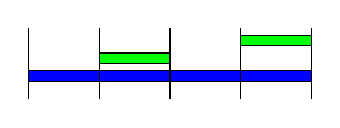
\begin{tikzpicture}[scale=.9]


\fill[blue] (0,.05) rectangle (4,.20);
\draw (0,.05) rectangle (4,.20);

\fill[green] (1,.30) rectangle (2,.45);
\draw (1,.30) rectangle (2,.45);

\fill[green] (3,.55) rectangle (4,.70);
\draw (3,.55) rectangle (4,.70);
 
\foreach \x in {0,1,2,3,4} {
    \draw (\x,-.2) -- (\x,.8);
}


\end{tikzpicture} 
\caption{Class 101a}
\end{figure}

\begin{figure}[h] \centering 
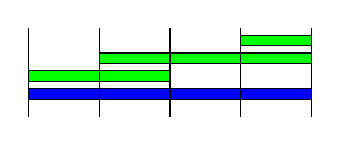
\begin{tikzpicture}[scale=.9]


\fill[blue] (0,.05) rectangle (4,.20);
\draw (0,.05) rectangle (4,.20);

\fill[green] (0,.30) rectangle (2,.45);
\draw (0,.30) rectangle (2,.45);

\fill[green] (1,.55) rectangle (4,.70);
\draw (1,.55) rectangle (4,.70);
 
\fill[green] (3,.80) rectangle (4,.95);
\draw (3,.80) rectangle (4,.95);
 
\foreach \x in {0,1,2,3,4} {
    \draw (\x,-.2) -- (\x,1.05);
}


\end{tikzpicture} 
\caption{Class 101b}
\end{figure}

As with the $110$ class, the members of $101$ can both be covered completely with 3 explanations, meaning 2 can always score $\frac23$ of the optimum score.

\subsubsection{Exhaustive Explanation Enumeration} \label{sec:exhaustiveEnumeration}

The next two classes can each only be drawn in one way and require some labeling and reasoning to get our $.655$ approximation factor.

\begin{figure}[h] \centering 
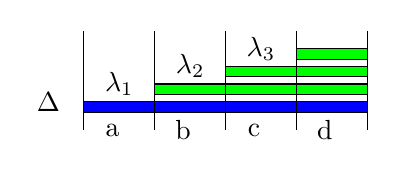
\begin{tikzpicture}[scale=.9]

\foreach \x in {0,1,2,3} {
    \fill[green] (\x,\x/4 +.05) rectangle (4,\x/4+.2);
    \ifnum \x = 0
      \fill[blue] (\x,\x/4 +.05) rectangle (4,\x/4+.2);
    \fi
    \draw (\x,\x/4 +.05) rectangle (4,\x/4+.2);

    \draw (\x,-.2) -- (\x,1.2);
}
\draw (4,-.2) -- (4,1.2);

\node (a) at (0+.4,-.2) {a};
\node (b) at (1+.4,-.2) {b};
\node (c) at (2+.4,-.2) {c};
\node (d) at (3+.4,-.2) {d};

\node (delta) at ( -.5,.2) {$\Delta$};
\node (l1)    at (.5,.45 ) {$\lambda_1$};
\node (l2)    at (1.5,.7 ) {$\lambda_2$};
\node (l3)    at (2.5,.95) {$\lambda_3$};

\end{tikzpicture} 
\caption{Class 111}
\end{figure}

\begin{figure}[h] \centering 
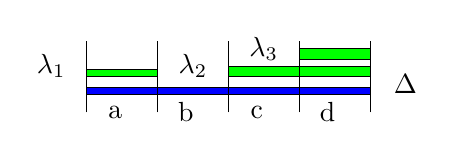
\begin{tikzpicture}[scale=.9]


\fill[blue] (0,.05) rectangle (4,.15);
\draw (0,.05) rectangle (4,.15);

\fill[green] (0,.30) rectangle (1,.40);
\draw (0,.30) rectangle (1,.40);

\foreach \x in {2,3} {
  \fill[green] (\x,\x/4 -.2) rectangle (4,\x/4-.05);
  \draw (\x,\x/4 -.2) rectangle (4,\x/4-.05);
}

\foreach \x in {0,1,2,3,4} {
    \draw (\x,-.2) -- (\x,.8);
}

\node (a) at (0+.4,-.2) {a};
\node (b) at (1+.4,-.2) {b};
\node (c) at (2+.4,-.2) {c};
\node (d) at (3+.4,-.2) {d};

\node (delta) at (4.5,.2 ) {$\Delta$};
\node (l1)    at (-.5,.45) {$\lambda_1$};
\node (l2)    at (1.5,.45) {$\lambda_2$};
\node (l3)    at (2.5,.70) {$\lambda_3$};

\end{tikzpicture} 
\caption{Class 011}
\end{figure}

The full score available from covering a subproblem of class $111$ is:

\begin{align*} 
S_{MAX} = &a \Delta + b \Delta + c \Delta + d \Delta + \hdots \\
& b \lambda_1 + c\lambda_1 + d\lambda_1 + \hdots \\
& c \lambda_2 + d \lambda_2 + d \lambda_3
\end{align*}

The set of maximal explanations for a subproblem of class $111$ would include all explanations that begin where a defect begins and end where one ends.  That set is: $ (0,4) (1,4) (2,4) (3,4)$.  There are $(^4_2) = 6$ possible explanation pairs to cover this region, and so we form a table.

The table, $C$ is $6 \times 10$, with each column representing one of our 6 possible explanation pairs, and each row corresponging to a term in the $S_{MAX}$ sum.  If $C(i,j) = 0$, neither of the explanations in pair $i$ covers term $j$ in the sum. Otherwise, $C(i,j) = 1$.

\begin{tabular}{l|llllll}
      & (0,4) & (0,4) & (0,4) & (1,4) & (1,4) & (2,4) \\
$s_j$ & (1,4) & (2,4) & (3,4) & (2,4) & (3,4) & (3,4) \\ \hline
$a\Delta$ & 1 & 1 & 1 & 0 & 0 & 0 \\
$b\Delta$ & 1 & 1 & 1 & 1 & 1 & 0 \\
$c\Delta$ & 1 & 1 & 1 & 1 & 1 & 1 \\
$d\Delta$ & 1 & 1 & 1 & 1 & 1 & 1 \\
$b \lambda_1$ & 1 & 0 & 0 & 1 & 1 & 0 \\
$c \lambda_1$ & 1 & 1 & 0 & 1 & 1 & 0\\
$d \lambda_1$ & 1 & 1 & 1 & 1 & 1 & 0 \\
$c \lambda_2$ & 0 & 1 & 0 & 1 & 0 & 1\\
$d \lambda_2$ & 0 & 1 & 1 & 1 & 0 & 1\\
$d \lambda_3$ & 0 & 0 & 1 & 0 & 1 & 1\\
\end{tabular}

For any column $i$, the score obtained by placing those two explanations is $\sum_j s_j C(i,j)$.  Because each $s_j$ is a product of $x \in \{ \delta \lambda_1, \lambda_2, \lambda_3 \}$ and $\alpha \in \{ a, b, c, d \}$, our problem can be reformulated as the quadratically constrained quadratic program (QCQP):

\begin{alignat*}{2}
  \text{minimize } & F \\
  \text{ subject to: } & \forall_j F \geq \sum_j s_j C(i,j) \\
                        & \sum_i s_i = 1 \\
                        & \sum_j \alpha_j = 1 \\
                        & \forall_{i>0} x_i \leq 1 \\
                        & 0 < \alpha_i < 1 \\
                        & 0 < x_i \\
\end{alignat*}

Our first constraint ensures that we are minimizing the highest score attainable by any legal combination of maximal explanations. The second constraint, $\sum_i s_i = 1$ scales the score we achieve in this interval, making $F$ the ratio of score we can get to score possible in this interval. The third constraint, $\sum_j \alpha_j = 1$ scales distance to allow for a unique solution to be found.  

The fourth constraint, $\forall_{i>0} x_i \leq 1$ guarantees that each defect $\lambda_k$ can only schieve a score of 1, with the exception of $\delta$. Since $\delta$ represents the sum of all defects that started before this span and end after it, it clearly should not be constrained.

For $d=2$, this QCQP can easily be typed into a computer algrbra system (i.e. Mathematica) or modeling language (like AMPL) and yields a solution of .705 for class $011$ and .655 for $111$.  As we are looking for the worse performing class, we see that in each 4 width subdivision, 2 explanations can score at least $65.5\%$ of the available score.

For $d > 2$, the process outlined in section~\ref{sec:exhaustiveEnumeration} is difficult to do by hand.  We wrote a computer program to solve this problem. Its subroutines:

\begin{enumerate}
\item Given the input $d$, generate all subproblem classes as $2d-1$ bit numbers.  (i.e. $111, 101$)
\item For each class, enumerate all possible matchings of defect beginning and defect end to find all members of a class. (i.e. $101a, 101b$)
\item Check if any set of $d+1$ explanations completely covers the class (since $\alpha$ is theorized to be $\leq \frac{d}{d+1}$).
\item For each of these class members, find the set $|E|$ of maximal explanations.  
\item Using quadratic programming, calculates the min-max of the score of $(^{|E|}_{\hspace{3pt}d})$ of these explanations.
\item Report as the approximation factor for $d$ the score from the worst performing class.
\end{enumerate}

We used the open source ipopt non-linear programming solver described in \cite{wachter2006implementation} to solve the many quadratic programs that this procedure generates.  Our numerical results follow:

\begin{tabular}{l|l}
$d$ & Lower Bound \\ \hline
2 & .655 \\ 
3 & .698 \\
4 & .736 \\
5 & .754 \\
6 & .773 \\
\end{tabular}

While these bounds are encouraging, the dynamic program runs in $O(|E|^{d})$.  Since we expect $|E| \geq 1000$, the dynamic program for $d=4$ is going to take of order an hour on modern hardware, and $d=5$ will take upwards of a month.

\subsection{Linear Programming Relaxation / Binary Programming} \label{sec:IP}

We are going to employ an LP relaxation in our numerical studies to determine how close to optimal our solution is.  We'll also see how frequently a cutting plane method can find a feasible, optimal solution to the integer program.

In order to turn our problem into an LP, we need to use defect primitives.  These were defined in section \ref{sec:definitions}.

With defect primitives in hand, we can define a linear program that maximizes the weighted sum of defect primitives explained.  The constraints are that each defect primitive is only explained if a covering explanation is in the set {\bf $E$}.  We have no more than $k$ explanations in {\bf $E$}.  Primitives can only be counted once for score.

Our variables are: 

$e_i$: 1 if explanation $E_i$ is in our explanation set, and 0 if not.

$p_{i,j}$: 1 if defect primitive $d_{i,j}$ is explained, 0 if it is not.

Note: $|d_{i,j}|$ and $|D_i|$ are constant lengths.

Without integer constraints, our LP relaxation is:
\begin{eqnarray*}
  \textrm{Maximize} &\sum_i \sum_j p_{i,j} \frac{|d_{i,j}|}{|D_i|} \\
  \textrm{Subject to:} &\\
  \forall_{i,j} p_{i,j} &\leq \sum_k e_k \cdot \theta(E_k \subseteq D_i \wedge d_{i,j} \subseteq E_K ) \\
  &\sum_i e_i \leq k \\
  &\forall_{i,j} p_{i,j} \leq 1 \\
  &\forall_{i,j} e_i \leq 1 \\
\end{eqnarray*}

Those integer constraints are:

\begin{eqnarray*}
  &\forall_{i,j} p_{i,j} \in \{0,1\} \\
  &\forall_{i,j} e_i  \in \{0,1\} \\
\end{eqnarray*}

\subsubsection{Total Unimodularity}

\begin{table*}[tbh]
\centering
\begin{tabular}{rrrr|rrrrrrrrrr}
$e_1$ & $e_2$ & $e_3$ & $e_4$ & $d_1$ & $d_2$ & $d_3$& $d_{1,1}$ & $d_{1,2}$ & $d_{1,3}$ & $d_{1,4}$ & $d_{1,5}$ & $d_{1,6}$ & $d_{1,7}$  \\
-1 &  0 &  0 &  0 & 1 & 0 & 0 & 0 & 0 & 0 & 0 & 0 & 0 & 0\\
 0 & -1 &  0 &  0 & 0 & 1 & 0 & 0 & 0 & 0 & 0 & 0 & 0 & 0\\
 0 &  0 & -1 &  0 & 0 & 0 & 1 & 0 & 0 & 0 & 0 & 0 & 0 & 0\\
 0 &  0 &  0 & -1 & 0 & 0 & 0 & 1 & 0 & 0 & 0 & 0 & 0 & 0\\
\cellcolor{gray}-1 &  \cellcolor{gray}0 &  \cellcolor{gray}0 & \cellcolor{gray}-1 & 0 & 0 & 0 & 0 & 1 & 0 & 0 & 0 & 0 & 0\\
 0 &  0 &  0 & -1 & 0 & 0 & 0 & 0 & 0 & 1 & 0 & 0 & 0 & 0\\
 \cellcolor{gray}0 & \cellcolor{gray}-1 &  \cellcolor{gray}0 & \cellcolor{gray}-1 & 0 & 0 & 0 & 0 & 0 & 0 & 1 & 0 & 0 & 0\\
 0 &  0 &  0 & -1 & 0 & 0 & 0 & 0 & 0 & 0 & 0 & 1 & 0 & 0\\
 \cellcolor{gray}0 &  \cellcolor{gray}0 & \cellcolor{gray}-1 & \cellcolor{gray}-1 & 0 & 0 & 0 & 0 & 0 & 0 & 0 & 0 & 1 & 0\\
 0 &  0 &  0 & -1 & 0 & 0 & 0 & 0 & 0 & 0 & 0 & 0 & 0 & 1\\
\cellcolor{gray} 1 & \cellcolor{gray} 1 & \cellcolor{gray} 1 & \cellcolor{gray} 1 & 0 & 0 & 0 & 0 & 0 & 0 & 0 & 0 & 0 & 0\\
\end{tabular}
\caption{Simple non-totally unimodular constraint matrix.}
\label{table:notUni}
\end{table*}

Were our formulation totally unimodular, the linear program would always guarantee an integer solution and merely coming up with this model would solve the problem.  Unfortunately this is not the case.  We will prove this by counterexample.

\begin{figure}[htb] 
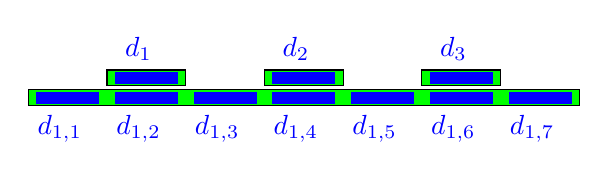
\begin{tikzpicture}[xscale=1,yscale=.25]

\fill[green] (0,2) rectangle (7,2.8);
\draw (0,2) rectangle (7,2.8);

\foreach \x in {1,2,3,4,5,6,7}
{
  \fill[blue] (\x-.9,2.1) rectangle (\x-.1,2.7);
  \node[blue] at (\x-.6,2.0) [below] {$d_{1,\x}$};
}

\foreach \x in {1,2,3}
{
  \fill[green] (2*\x-1,3) rectangle (2*\x-1+1,3.8);
  \draw (2*\x-1,3) rectangle (2*\x-1+1,3.8);
  
  \fill[blue] (2*\x-1+.1,3.1) rectangle (2*\x-1+.9,3.7);
  \node[blue] at (2*\x-1+.4,3.8) [above] {$d_{\x}$};
}

\end{tikzpicture} 
\caption{Simple non-totally unimodular defect set.}
\label{fig:notUni}
\end{figure}

The constraint matrix for the defect set and associated maximal explanations in figure~\ref{fig:notUni} is shown in table~\ref{table:notUni}. We use Camion's necessary and sufficient condition for total unimodularity from \cite{camion1965} to prove this constraint array is not totally unimodular.  We quote that theorem below:

\begin{thm}
Matrix A is totally unimodular if and only if for every (square) Eulerian submatrix $A_j^I \sum_{i\in I} \sum_{j \in J} A^i_j = 0$ mod 4.
\end{thm}

The highlighted cells from our constraint matrix form the following $4 \times 4$ square submatrix:

\begin{tabular}{rrrr}
-1 &  0 &  0 & -1 \\
 0 & -1 &  0 & -1 \\
 0 &  0 & -1 & -1 \\
 1 &  1 &  1 &  1 \\
\end{tabular}  

This submatrix is Eulerian since the sum of elements in each of its rows and columns are even, but the sum of all elements is $-2$, a number that is not divisible by $4$.  By Camion's theorem, this constraint matrix is not totally unimodular, so in general we cannot assume that any of our constraint matrices will be totally unimodular.

\section{Algorithm Bakeoff}

While the only algorithms with calculated bounds are the dynamic programming algorithm, and the Binary Programming algorithm (optimal when a solution is found), we tested our algorithms' performance on randomly generated instances. The algorithms tested were:

\texttt{greedyExplanationCover} The greedy algorithm described in section~\ref{sec:greedy}.  For each of its k steps, places the highest scoring explanation given the explanations already placed.

\texttt{1-OPT} A natural improvement to greedy where the output is improved by a series of single explanation exchanges.  It is greedy itself, choosing the best single exchange at each step and terminating once there are no exchanges that will improve the score.

\texttt{Depth 1 Dynamic Program} The approach from section~\ref{sec:DP}, uses a dynamic program to solve this problem.  The dynamic program's solution is limited to the space of all solutions where no 2 explanations overlap.

\texttt{Depth 2 Dynamic Program} This algorithm, described in section~\ref{sec:dpFixedDepth}, uses a dynamic program to solve this problem.  The dynamic program's solution is limited to the space of all solutions where no 3 explanations overlap.

\texttt{Integer Program Solution} Implements the Binary program from section~\ref{sec:IP} and lets the COIN-OR's OsiClpSolver (as described in \cite{COIN-OR}) use branch and bound methodology to get a solution.

\subsection{Methods}

Because purely random samples are unlikely to find even a local minimum, we modified the GAlib genetic algorithm library \cite{GAlib} to minimize the performance ratios of our algorithms.  A gene consisted of $2N$ integers from $[0,100]$.  Each consecutive pair of endpoints was made into a defect.  

We started with a completely random population, and used a steady state GA with sexual reproduction characterized by two point crossover.  We wrote a custom mutation routine that selected one of the following three randomization operations:

{\it Point flip:} This looped through the entire gene and with constant probability $p$ per endpoint, changed that value to a random number in $[0,100]$.  

{\it Neighbor swap:} Loop through the entire gene, and with probability $p$ per defect, swapped an endpoint of defect $i$ with an endpoint of defect $j$.

{\it Random inversions:} For each position $i$ in the genome, with probability $p$, generate a random number $x$ in $[1,2k-i]$ and reverse the order of the next $x$ alleles.  

We made the objective function to minimize the performance of each algorithm in turn, and ran it for 10,000 generations with a population of 400.  

\subsection{$N=K$ Results}

When $N=K$, the trivially optimal solution would be one explanation identical to each defect.  Since 1-OPT and IP were uniformly optimal for these cases, they are not shown.

\vspace{6pt}

\begin{tabular}{l|llll}
{\bf Alg.} & DP 1 & Greedy & DP 2 \\ \hline
{\bf $(N,K)$ } \\
(2, 2) & 0.50 & 0.75  & 1    \\
(3, 3) & 0.67 & 0.79  & 0.90 \\
(4, 4) & 0.75 & 0.78  & 0.90 \\
(5, 5) & 0.75 & 0.82  & 0.91 \\
(6, 6) & 0.77 & 0.82  & 0.91 \\
\end{tabular}

\subsection{$N \leq k$}

We then held $N$ steady, and varied $k$. Here we had to use the LP relaxation in place of an {\it a priori } OPT:

\begin{figure}[ht!] \centering
  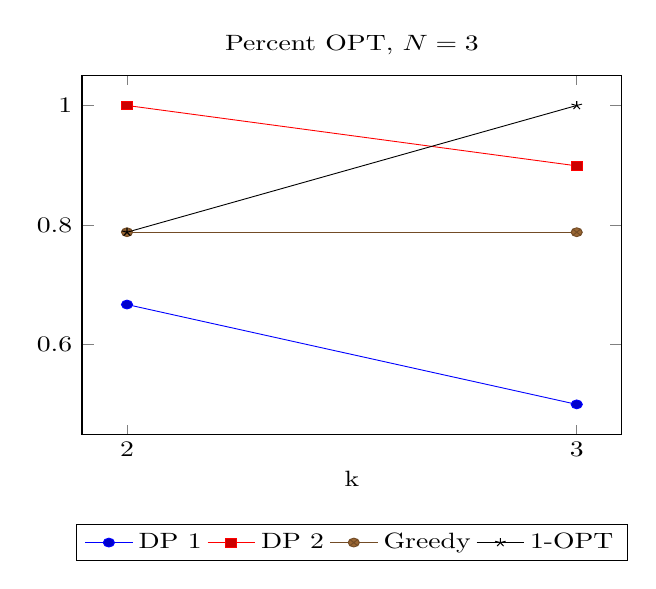
\begin{tikzpicture}[yscale=.8]
    \begin{axis}[ title={Percent OPT, $N=3$}, 
        xlabel=k,
        /pgfplots/xtick={2,...,5},
        legend style={at={(.5,-.25)},anchor=north,legend columns=4},
      ]
      \addplot+[smooth] coordinates {(2, 0.667) (3, 0.5  )};    
      \addplot+[smooth] coordinates {(2, 1.00 ) (3, 0.899)};    
      \addplot+[smooth] coordinates {(2, 0.788) (3, 0.788)};    
      \addplot+[smooth] coordinates {(2, 0.788) (3, 1.0  )};    
      \legend {DP 1, DP 2, Greedy,  1-OPT}
    \end{axis}
  \end{tikzpicture}
  \caption{Results for placing $2-3$ explanations to cover $3$ defects.}
\end{figure}
\FloatBarrier

Here we see what will become the overriding theme.  A one depth dynamic program is strictly inferior to the 2 depth DP, and worst performer overall.  As expected in light of greedy being a preprocessing step to 1-OPT, 1-OPT dominates greedy.  The 2 depth dynamic program outscores 1-OPT for low $k$ and gives up that lead as $k$ increases.

\begin{figure}[ht!] \centering
  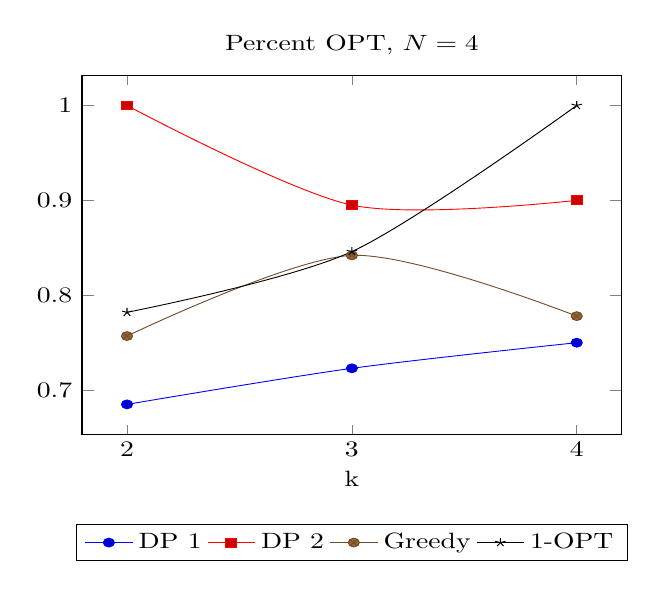
\begin{tikzpicture}[yscale=.8]
    \begin{axis}[ title={Percent OPT, $N=4$}, 
        xlabel=k,
        /pgfplots/xtick={2,...,5},
        legend style={at={(.5,-.25)},anchor=north,legend columns=4},
      ]
      \addplot+[smooth] coordinates {(2, 0.685) (3, 0.723) (4, 0.75 )};    
      \addplot+[smooth] coordinates {(2, 1.00 ) (3, 0.895) (4, 0.9 )};    
      \addplot+[smooth] coordinates {(2, 0.757) (3, 0.842) (4, 0.778 )};    
      \addplot+[smooth] coordinates {(2, 0.782) (3, 0.846) (4, 1.0 )};    
      \legend {DP 1, DP 2, Greedy,  1-OPT}
    \end{axis}
  \end{tikzpicture}
  \caption{Results for placing $2-4$ explanations to cover $4$ defects.}
\end{figure}
\FloatBarrier
The exact same pattern holds, with our algorithms from worst to best being one depth dynamic program, greedy and the 1-OPT / 2 depth tie.

\begin{figure}[ht!] \centering
  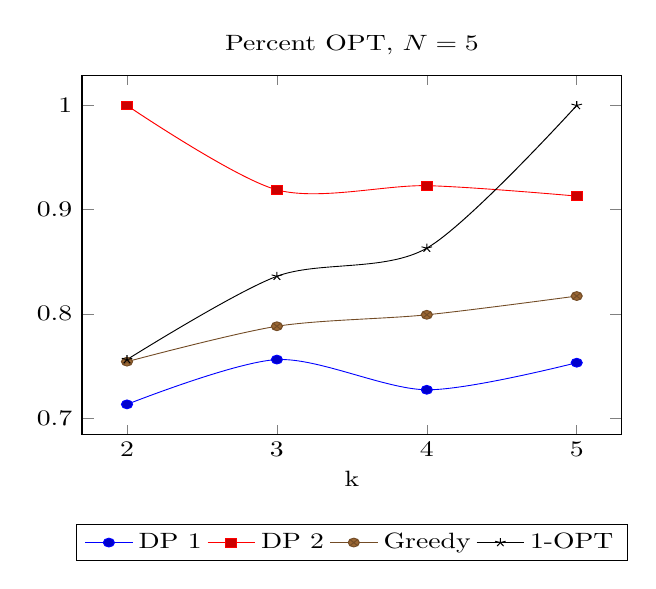
\begin{tikzpicture}[yscale=.8]
    \begin{axis}[ title={Percent OPT, $N=5$}, 
        xlabel=k,
        /pgfplots/xtick={2,...,5},
        legend style={at={(.5,-.25)},anchor=north,legend columns=4},
      ]
      \addplot+[smooth] coordinates {(2, 0.713) (3, 0.756) (4, 0.727) (5,0.753)};    
      \addplot+[smooth] coordinates {(2, 1.00 ) (3, 0.919) (4, 0.923) (5, 0.913)};    
      \addplot+[smooth] coordinates {(2, 0.754) (3, 0.788) (4, 0.799) (5,0.817)};    
      \addplot+[smooth] coordinates {(2, 0.756) (3, 0.836) (4, 0.863) (5,1) };    
      \legend {DP 1, DP 2, Greedy,  1-OPT}
    \end{axis}
  \end{tikzpicture}
  \caption{Results for placing $2-5$ explanations to cover $5$ defects.}
\end{figure}

\FloatBarrier

Here, while the rankings don't change, the 2-depth dynamic program held its lead for all but the $N=K$ case.  Considering that 1-OPT will always find the optimal solution in an $N=k$ case, and that real life scenarios are characterized by $N>>k$, this result strongly suggests that the 2 depth dynamic program outperforms the other three heuristics.  

The clear winner was binary programming (not shown).  In all but 4 of the genome evaluations (out of ~1.6 million), the MILP solver from COIN-OR produced an optimal output.  If it scales well for problems of real world applicationsize, it would be the best algorithm to use in practice.

\FloatBarrier

\subsection{Timing Data}

To illustrate algorithm running times on smallscale problems, we generated 1024 random defect sets of size $N \in \{4 8 16\}$ and had each algorithm place $K = \{ N, N/2, N/4\}$ explanations.  The timing results follow:

\begin{figure}[ht!] \centering
  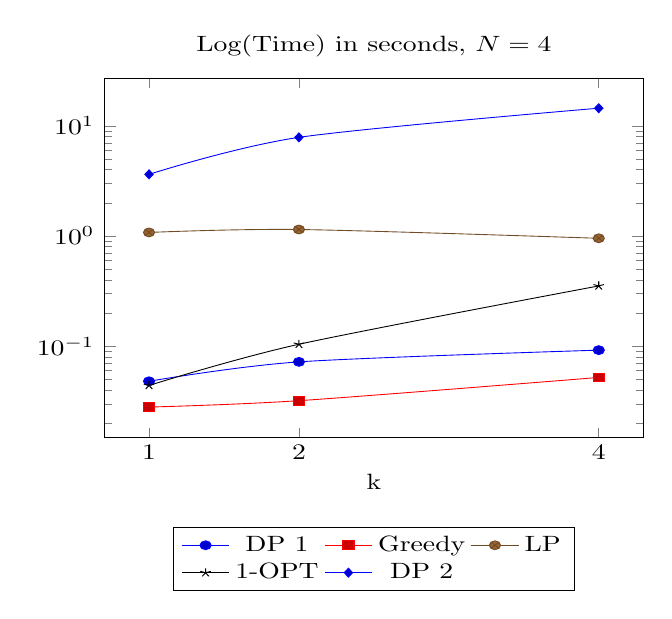
\begin{tikzpicture}[yscale=.8]
    \begin{axis}[ title={Log(Time) in seconds, $N=4$}, 
        ymode=log,
        xlabel=k,
        /pgfplots/xtick={1,2,4},
        legend style={at={(.5,-.25)},anchor=north,legend columns=3},
      ]
      \addplot+[smooth] coordinates {(1, 0.048) (2,0.072) (4, 0.092) };    
      \addplot+[smooth] coordinates {(1, 0.028) (2,0.032) (4, 0.052) };    
      \addplot+[smooth] coordinates {(1, 1.076) (2,1.144) (4, 0.952) };    
      \addplot+[smooth] coordinates {(1, 0.044) (2,0.104) (4, 0.352) };    
      \addplot+[smooth] coordinates {(1, 3.624) (2,7.848) (4,14.436) };    
      \legend {DP 1, Greedy,  LP, 1-OPT, DP 2}
    \end{axis}
  \end{tikzpicture}
  \caption{Time to place $k$ explanations to cover 4 defects.}
\end{figure}
\FloatBarrier

Even for small cases, the depth 2 dynamic program is more than 10 times slower than any other algorithm.  Since it scales as $O(kn^{2+k})$, this algorithm will quickly become impractical.  We will devote a chart to its scaling, but omit it from the rest of the timing plots.

\begin{figure}[ht!] \centering
  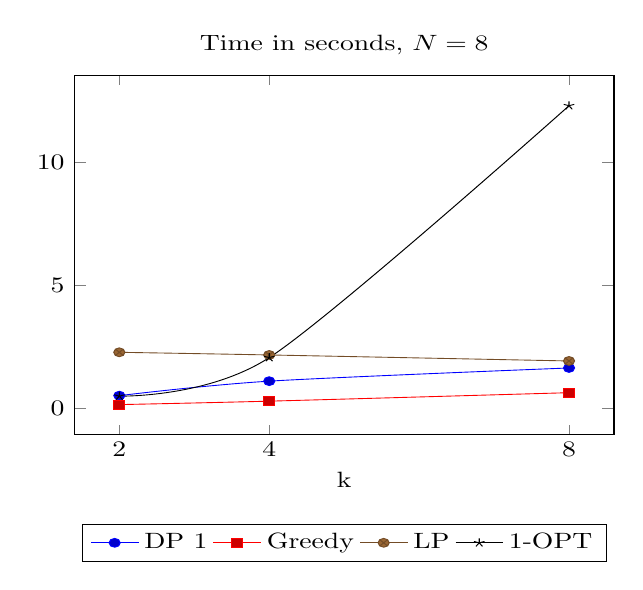
\begin{tikzpicture}[yscale=.8]
    \begin{axis}[ title={Time in seconds, $N=8$}, 
        xlabel=k,
        /pgfplots/xtick={2,4,8},
        legend style={at={(.5,-.25)},anchor=north,legend columns=4},
      ]
      \addplot+[smooth] coordinates {(2, 0.508) (4,1.096) (8,1.632) };    
      \addplot+[smooth] coordinates {(2, 0.144) (4,0.284) (8,0.628) };    
      \addplot+[smooth] coordinates {(2, 2.268) (4,2.160) (8,1.916) };    
      \addplot+[smooth] coordinates {(2, 0.488) (4,2.052) (8,12.280) };    
      \legend {DP 1, Greedy,  LP, 1-OPT}
    \end{axis}
  \end{tikzpicture}
  \caption{Time to place $k$ explanations to cover 8 defects.}
\end{figure}

1-OPT's scaling is so much greater than the other algorithms that it is masking the story.  The dynamic program and greedy algorithm are both requiring more time as $k$ increases while the LP, surprisingly, requires less.

\begin{figure}[ht!] \centering
  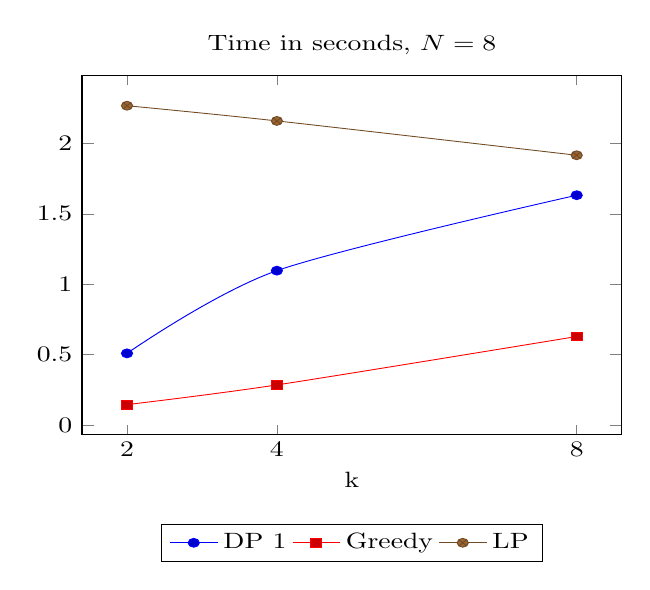
\begin{tikzpicture}[yscale=.8]
    \begin{axis}[ title={Time in seconds, $N=8$}, 
        xlabel=k,
        /pgfplots/xtick={2,4,8},
        legend style={at={(.5,-.25)},anchor=north,legend columns=4},
      ]
      \addplot+[smooth] coordinates {(2, 0.508) (4,1.096) (8,1.632) };    
      \addplot+[smooth] coordinates {(2, 0.144) (4,0.284) (8,0.628) };    
      \addplot+[smooth] coordinates {(2, 2.268) (4,2.160) (8,1.916) };    
      \legend {DP 1, Greedy,  LP}
    \end{axis}
  \end{tikzpicture}
  \caption{Time to place $k$ explanations to cover 8 defects (without 1-OPT).}
\end{figure}

\begin{figure}[ht!] \centering
  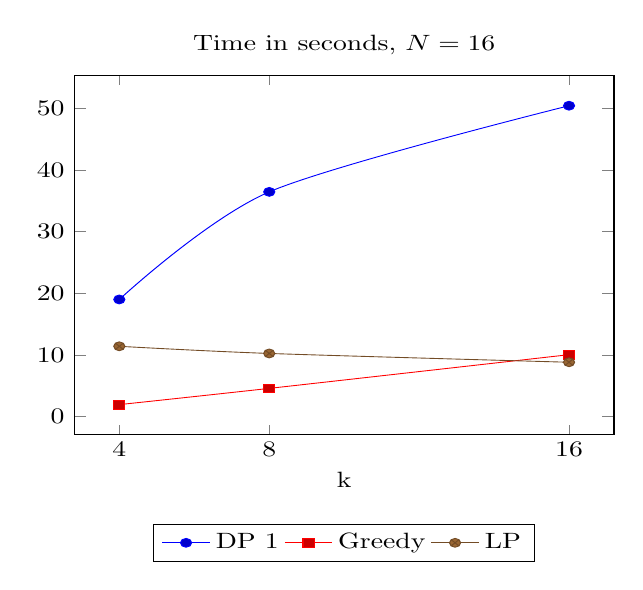
\begin{tikzpicture}[yscale=.8]
    \begin{axis}[ title={Time in seconds, $N=16$}, 
        xlabel=k,
        /pgfplots/xtick={4,8,16},
        legend style={at={(.5,-.25)},anchor=north,legend columns=4},
      ]
      \addplot+[smooth] coordinates {(4,19.000) (8,36.452) (16, 50.432) };    
      \addplot+[smooth] coordinates {(4, 1.940) (8, 4.572) (16, 10.040) };    
      \addplot+[smooth] coordinates {(4,11.400) (8,10.240) (16,  8.812) };    
      \legend {DP 1, Greedy,  LP}
    \end{axis}
  \end{tikzpicture}
  \caption{Time to place $k$ explanations to cover 16 defects.}
\end{figure}

The $N=16$ and $N=32$ graphs tell the same story. Greedy scales linearly with $k$, the LP takes marginally less time as $k$ increases and the DP scales as either $\sqrt{k}$ or $\log{k}$ but with large enough $n$ dependent scaling to be slow

\begin{figure}[ht!] \centering
  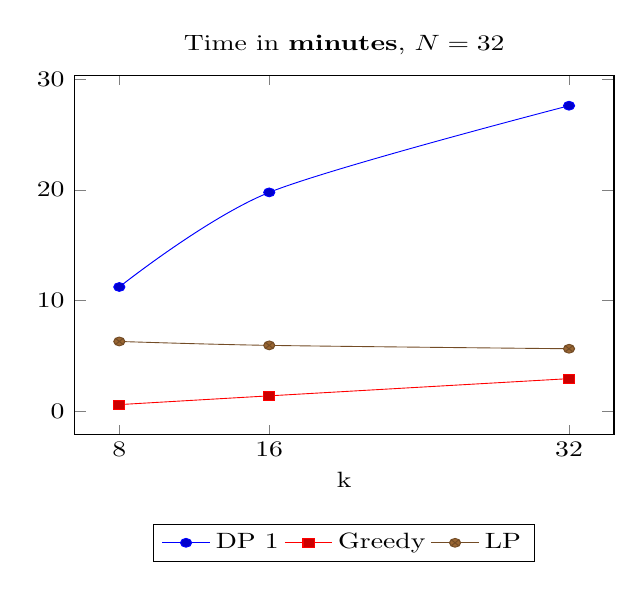
\begin{tikzpicture}[yscale=.8]
    \begin{axis}[ title={Time in {\bf minutes}, $N=32$}, 
        xlabel=k,
        /pgfplots/xtick={8,16,32},
        legend style={at={(.5,-.25)},anchor=north,legend columns=4},
      ]
      \addplot+[smooth] coordinates {(8,11.217) (16,19.764) (32, 27.598) };    
      \addplot+[smooth] coordinates {(8, 0.586) (16, 1.377) (32,  2.932) };    
      \addplot+[smooth] coordinates {(8, 6.293) (16, 5.939) (32,  5.634) };    
      \legend {DP 1, Greedy,  LP}
    \end{axis}
  \end{tikzpicture}
  \caption{Time to place $k$ explanations to cover 32 defects.}
\end{figure}

\FloatBarrier

A log-log linear regression on the $k$ dependence of the 1-OPT algorithm shows that its dependence on $k$ is approximately $O(k^{2.5})$.  For moderate values of $k\leq 100$, this may prove acceptable for use in the field. 


\subsubsection{2-Depth DP Timing}

\begin{figure}[ht!] \centering
  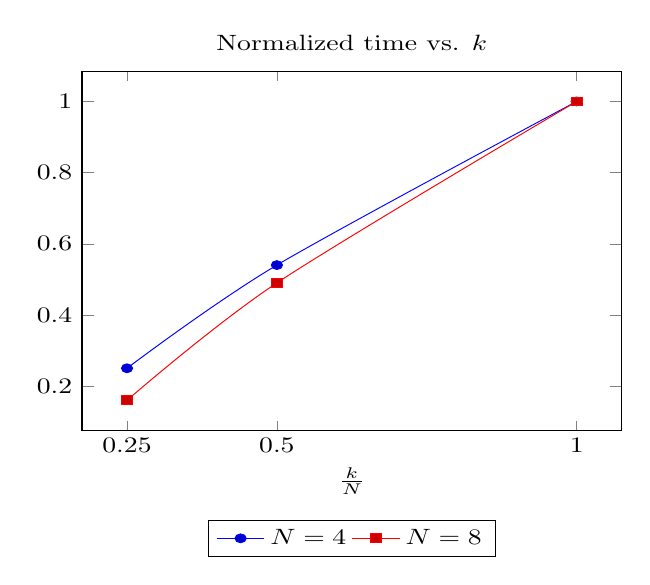
\begin{tikzpicture}[yscale=.8]
    \begin{axis}[ title={Normalized time vs. $k$}, 
        xlabel=$\frac{k}{N}$,
        /pgfplots/xtick={.25,.5,1},
        legend style={at={(.5,-.25)},anchor=north,legend columns=2},
      ]
      \addplot+[smooth] coordinates {(.25,0.25) (.5,0.54) (1,1) };    
      \addplot+[smooth] coordinates {(.25,0.16) (.5,0.49) (1,1) };    
      \legend {$N=4$, $N=8$}
    \end{axis}
  \end{tikzpicture}
  \caption{Timing data for the 2-depth dynamic program. Note that time is normalized by the duration of the $N=k$ call.}
\end{figure}

The running time dependence on $k$ for the 2-Depth dynamic program is exactly as it should be: linear.

\begin{figure}[ht!] \centering
  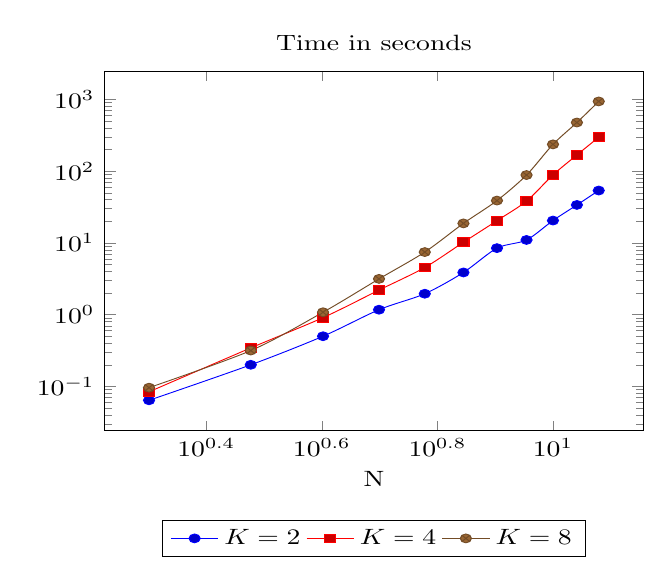
\begin{tikzpicture}[yscale=.8]
    \begin{axis}[ title={Time in seconds}, 
        xlabel=N,
        ymode=log,
        xmode=log,
        legend style={at={(.5,-.25)},anchor=north,legend columns=3},
      ]
      \addplot+[smooth] coordinates {(2, 0.064) (3, 0.200) (4, 0.500) (5, 1.172) (6, 1.956) (7, 3.872) (8, 8.448) (9, 10.992) (10, 20.5) (11, 33.8) (12, 53.7)};
      \addplot+[smooth] coordinates {(2, 0.084) (3, 0.344) (4, 0.908) (5, 2.2) (6, 4.54) (7, 10.2) (8, 20.4) (9, 38.3) (10, 88.6) (11, 168) (12, 297)};
      \addplot+[smooth] coordinates {(2, 0.096) (3, 0.316) (4, 1.08) (5, 3.15) (6, 7.45) (7, 18.7) (8, 38.9) (9, 88.3) (10, 236) (11, 476) (12, 937)};
    \legend {$K=2$, $K=4$, $K=8$}
    \end{axis}
  \end{tikzpicture}
  \caption{Timing data for the 2-depth dynamic program as a function of $N$}
\end{figure}

On the other hand, the pessimistic $O(kN^{k+2})$ upper bound on running time is exactly that, pessimistic. The best fitting line's slope for the log-log plot with $k=2$ was 3.78, and for $k=4$ it was 4.26, and 5.21 for $k=8$. We hypothesize that these coefficients are below the worst case powers of $4, 6$ and $10$ because that bound occurs when our defect set is of depth $O(N)$ for the majority of times we encounter an endpoint. 

If this hypothesis holds, it's possible that the structure of real data will allow for even better running times for the dynamic programming algorithm than did our synthetic data.

\FloatBarrier
\section{Conclusions}

We studied a number of candidate heuristics for the DNA copy number analysis problem.  Our most powerful approaches were a binary programming formuation of the problem and dynamic programming based PTAS. The PTAS has both a stronger theoretical grounding and performance guarantees, but its running time is prohibitively expensive.

Fortunately, the binary programming formulation solved with a freeware MILP had a very acceptable running time for problems of modest size.  It is our recommendation that researchers, specifically those who implemented the CORE product referenced in \cite{krasnitz2013target}, utilize this optimization method in place of their current greedy approach.


\chapter{The Waiter Problem in One Dimension}{
\begin{centering}
\par{\it James Zuber}

\par{\large \bf Summary:}

\end{centering}

\par{The waiter problem is a discrete packing problem where the objective is to contain the partial centers of mass of objects placed on a line within a small interval. We introduce the problem, prove its NP completeness, and present both a bound on performance and a 2.7 factor approximation heuristic to solve the problem.}
}

\section{Introduction}

The waiter problem is fairly easy to define.  Given a set $x_i \in X$ of unit point masses, we seek an ordering $\pi_i$ that optimizes a measurement on the partial centers of mass $C_j = \frac{\sum_{i=1}^j x_{\pi_i} }{ j }$. 

The measurement that we choose to optimize over is the length of the continuous interval $[L,R]$ that contains the set of $C_j$.  Other measurements proposed.  were the radius of a symmetric interval $[-r,r]$ containing all $C_j$, and the decision version of this problem: can the masses $x_i$ be placed in such an order that the partial center of mass never leaves the given interval $[A,B]$.  

Any input set $y$ can be transformed to have a final center of mass at 0 and  $\max |x_i| = 1$,  with the following transformation: $y_i \rightarrow \frac{y_i - \bar{y} }{\max(|y_i| - \bar{y}) }$.

\section{Literature Review}


While the problem that we are solving is novel, it is closely related to two well researched problems in the literature.  The first class of problems ask how to best pack one dimensional boxes into one dimensional containers.  

In \cite{mathur1998integer}, the problem under consideration is to pack one dimensional boxes into a container in such away that the center of mass is as close as possible to a target point.  This differs from our problem because the center of mass after each box is placed is never considered.  Optimizing the final position was worked on a few years earlier in \cite{amiouny1992balanced}, who showed it to be strongly NP hard by a reduction from 3 partition. They used the obvious idea of sorted orderings that we'll heavily rely on in this paper.  Another notable example of box packing was seen in \cite{davies1999weight} where they generalized the final position problem to be two dimensional, thus introducing an added complexity layer of closest packing (in addition to weight balance).

We see another approach to the packing problem in \cite{fasano2004mip} where he showed a mixed integer programming model whose answer would be an optimal packing of boxes.  Recently, a similar mixed integer programming approach was used in the practical application  of loading cargo airplanes \cite{limbourg2012automatic}.  

While the above are simliar to our problem, they all differ by not requiring that the center of mass be measured and constrained with each additional weight added.  A problem that requires such a constraint check at each step is {\it compact vector summation} or CVS. 

In CVS the problem is to specify an order to sum a number of $k-$dimensional vectors and keep every partial sum within a $k-$dimensional ball of fixed radius. In \cite{sevast1994some} we find an excellent summary of results in CVS and their application to job scheduling problems, this is updated with further results in \cite{sevastianov1998nonstrict}.  Because of the similarity between ours and the job scheduling problem, many of the heuristic approaches referenced in \cite{framinan2004review} and \cite{gupta2006performance} can be translated directly into heuristics for our problem, though we should be careful as certain bad cases for CVS \cite{chelidze2010greedy} are trivial in our problem.

\section{NP Completeness}

The waiter problem is NP complete, and the reduction is from 3-partition.  But before we prove this, we require one simple lemma.

\begin{lem} \label{lem:zerosChangeNothing} 
Placing a point at 0 (the final center of mass) never reduces the number of legal future moves.  
\end{lem}

\begin{proof}
When we place a point $x_{\pi_n}$, it will cause our center of mass to leave the current interval $[L, R]$ if either:

\begin{align*} 
\sum_{i=1}^{n-1} x_{\pi_i} + x_{\pi_n} &> n R \\
\sum_{i=1}^{n-1} x_{\pi_i} + x_{\pi_n} &< n L
\end{align*}

In other words, all legal values for the point $x_{\pi_n}$ lie in the interval $[ n L - \sum_{i=1}^{n-1} x_{\pi_i}, n R - \sum_{i=1}^{n-1} x_{\pi_i}] $

If our original sum over $n$ elements contained none with a value of zero, and our new sums contain $k$ elements with a value or zero, then the new inteval of all legal values is:

\begin{eqnarray*}
\Sigma &=& \sum_{i=1}^{n-1} x_{\pi_i} + \sum_{j=1}^k 0 \\
x_{\pi_n} &\leq& (n+k) R - \Sigma \\
x_{\pi_n} &\geq& (n+k) L - \Sigma \\
x_{\pi_n} &\in& [ (n+k) L - \Sigma, (n+k) R - \Sigma ]
\end{eqnarray*}

$\forall L, R$ with $L \leq R$ this is larger than our initial range of:

\begin{equation*}
x_{\pi_n} \in [ (n L - \Sigma, n R - \Sigma ]
\end{equation*}

Since our final center of mass is located at 0, and must be contained in our interval, we know that $L\leq 0$ and $R\geq 0$ so our initial range of values is a subinterval of the range allowed after placing the zeros.
\end{proof}

\begin{thm}\label{thm:completeness}
Given an instance of 3-partition where $ |x_i| = 3N, \forall_i \frac{1}{4} < x_i < \frac{1}{2} $, we can reduce it to an instance of the 1 dimensional waiter problem in polynomial time.  
\end{thm}

\begin{proof}
Our set of weights will fall into 3 categories.  There will be $M$ masses to place at 0 (which will be the final center of mass), there will be $N$ masses to place at $-1$ and the remaining $3N$ masses will all be placed at the positions $x_i$ corresponding to our 3-partition instance.

By lemma \ref{lem:zerosChangeNothing}, we can say that instead of requiring a non-polynomial reduction where $M$, the number of weights located at point 0, wasn't polynomial in input size and required we have that many weights in the instance, we can instead place those $M$ weights in $ O(1) $ time and tackle the remaining $ 3N + N$ weights in our reduction.

In order to remain in the interval $[0, \frac{1}{M}]$, whenever we seek to place one of our $x_i = -1$ weights, the running sum must be exactly 1.

\begin{eqnarray*}
\Sigma &=& \sum_{i=1}^{n-1} x_{\pi_i} + \sum_{j=1}^M 0 \\
x_i &\leq& (n+M) R - \Sigma \\
x_i &\leq& \frac{n}{M} + \frac{M}{M}- \Sigma = 1 - \Sigma \\
x_i &\geq& (n+M) L - \Sigma = 0 - \Sigma \\
x_i &\in& [ - \Sigma, 1 - \Sigma ]
\end{eqnarray*}

Positive $x_i$ weights can be placed whenever $x_i + \Sigma < 1$ and the negative values can be placed whenever $ -1 \in [\Sigma, 1-\Sigma] $, or $ \Sigma >= 1$.  But if $ \Sigma > 1$, we have the center of mass $ C = \frac{\Sigma}{k+M} \approx \frac{\Sigma}{M} > \frac{1}{M}$ where the approximation approaches equality as $ M \rightarrow \infty$.

This means our negative weights can only be placed when $\Sigma = 1$, i.e. when three positive masses have been placed that sum to 1.  Deciding if this can be repeated $N$ times is exactly the 3-partition question, which is NP-hard.
\end{proof}

The requirement that $\frac{\Sigma}{n+M} \leq \frac{1}{M}$ for all $\Sigma$ can allow us to set a lower bound for $M$.  As the greatest value $k$ will hold is $4n$, this gives us the requirement that:

\begin{equation*}
\Sigma \leq 1 + \frac{4n}{M}
\end{equation*}

TO ensure this is never violated, we find the smallest sum of 3 or 4 $x_i$ that is strictly greater than 1 and call this sum $1+\epsilon$.  When $\epsilon > \frac{4n}{M}$, all sums of 3 elements that are greater than $1$ are greater than $1 + \frac{k}{M}$ for all $k\leq 4n$.  

\section{Analytical Bounds}

\subsection{Naive Bound}

Throughout this section, we are requiring that $ \sum_i x_i = 0 $, an assumption that can be satisfied by transforming any input set $ y_i $ into $ x_i = y_i - \bar{y}$. 

We will show that $|R-L| \geq \frac{|x_i|}{i} $ is a naive lower bound on the optimum difference between the left and right endpoint of the interval containing the center of mass (hereafter $ C_i \in [ L, R ] $) if our masses are sorted by distance from the origin. 

Observation:

Adding a new point moves the current center of mass according to:

\begin{eqnarray*}
c_i = \frac{ x_i + \sum_{j=1}^{i-1} x_j }{ i } \\ 
c_i = \frac{ (i-1) c_{i-1}}{i} + \frac{x_i }{ i }  \\
c_i - c_{i-1} = \frac{x_i - c_{i - 1} }{ i } \\
|c_i - c_{i-1}| = \Delta C \leq |R - L|
\end{eqnarray*}

\begin{lem} \label{lem:matchSignNaive}
If $\textrm{sign}(c_i) = \textrm{sign}(c_{i-1})$ then $|R - L| \geq \frac{x_i}{i}$
\end{lem}

\begin{proof}
Continuing from above:

\begin{eqnarray*}
c_i - c_{i-1} = \frac{x_i - c_{i - 1} }{ i } \\
c_i = c_{i-1}( \frac{i-1}{i}) + \frac{x_i }{ i } \\
\big|c_i\big| = \big|c_{i-1} (\frac{i-1}{i}) + \frac{x_i }{ i }\big| \\
S = \textrm{sign}(c_{i-1} )*\textrm{sign}(x_i) \\
\big|c_i\big| = \big|c_{i-1} \big( \frac{i-1}{i} \big)\big| + S\big|\frac{x_i}{ i }\big|
\end{eqnarray*}

There are two cases:

Case 1, $\textbf{S = +1}$: 

\begin{eqnarray*}
\big|c_i\big| = \big|c_{i-1} \big( \frac{i-1}{i} \big) \big| + \big|\frac{x_i}{i}\big| \\
\rightarrow \big|c_i\big| \geq \big|\frac{x_i}{i}\big| \\ 
\big|R-L\big| \geq \big|c_i\big| \textrm{By definition of } R,L \\
\rightarrow \big|R-L\big| \geq \big|\frac{x_i}{i}\big|
\end{eqnarray*}

Case 2, $\textbf{S = -1}$: 

\begin{eqnarray*}
\big|c_i\big| = \big|c_{i-1} \big( \frac{i-1}{i} \big)\big| - \big|\frac{x_i}{i}\big| \\
\big|\frac{x_i}{i}\big| + \big|c_i\big| = \frac{i-1}{i}\big|c_{i-1}\big|  \\
\big|c_{i-1}\big| = \frac{i}{i-1}\big|\frac{x_i}{i}\big| + \frac{i}{i-1}\big|c_i\big| \\
\big|c_{i-1}\big| \geq = \frac{i}{i-1}\big|\frac{x_i}{i}\big| \\
\rightarrow \big|c_{i-1}\big| \geq \big|\frac{x_i}{i}\big| \\
\big|R-L\big| \geq \big|c_{i-1}\big| \textrm{By definition of } R,L \\ 
\rightarrow \big|R-L\big| \geq \big|\frac{x_i}{i}\big|
\end{eqnarray*}
\end{proof}

\begin{lem} \label{lem:diffSignNaive}
If $\textrm{sign}(c_i) \neq \textrm{sign}(c_{i-1})$ then $\big|R - L\big| \geq \frac{x_i}{i}$
\end{lem}

\begin{proof}
First, $\textrm{sign}(c_i) = \textrm{sign}(x_i)$  is trivially true as a positive $c_i$ can't be the sum of two negative numbers, and conversely a negative $c_i$ can't be the sum of two positive numbers.  Then we continue:

\begin{eqnarray*}
c_i = c_{i-1}\frac{i-1}{i} + \frac{x_i }{ i } \\ 
c_i - c_{i-1} = \frac{x_i}{i} - \frac{c_{i-1}}{i} \\
\big|c_i - c_{i-1}\big| = \big|\frac{x_i}{i} - \frac{c_{i-1}}{i}\big| \\
\big|c_i - c_{i-1}\big| = \big|\frac{x_i}{i}\big| + \big|\frac{c_{i-1}}{i}\big| \\
\big|c_i - c_{i-1}\big| \geq \big|\frac{x_i}{i}\big|  \\
\big|R-L\big| \geq \big|c_i - c_{i-1}\big| \textrm{By definition of } R,L \\
\big|R-L\big| \geq \big|\frac{x_i }{ i }\big|
\end{eqnarray*}

\end{proof}

By combining Lemmas \ref{lem:matchSignNaive} and \ref{lem:diffSignNaive}, we get:

\begin{thm} \label{thm:naiveBound}
For any ordering of $x_i$ the interval containing the center of mass satisfies: $\forall_i \big|R-L\big| \geq \frac{\big|x_i\big|}{i} $
\end{thm}

\begin{cor} \label{cor:naiveBound}
For any valid solution to the waiter problem, $|R-L| \geq \frac{|x_i|}{i}$ where $x_i$ is the mass whose position has the $i^{th}$ smallest magnitude.
\end{cor}

\subsubsection{Non-tightness of Naive Bound} \label{subs:naiveCounter}

The above bound is not particularly tight, as is evidenced by the following counterexample:

Allow the first $k$ $x_i$ to all be positive and have values of $i$.  Let $ x_{k-1} = -k $ and then require $ \forall_{ i > k}, -1 \leq \frac{x_i}{i} \leq 0 $ giving us a value of 1 for our naive bound on interval width.

The actual center of mass achieved by placing the masses in this order is: $ c_k = \frac{1}{k} \sum_{i=1}^k i = \frac{k-1}{2} $.

The optimal center of mass interval is shorter than this, as we can add positive weights in order until $ c_l = \frac{k}{l} $ which occurs approximately when $ \frac{l^2 - l}{2} = k \rightarrow l \approx 2\sqrt{k} $. This gives us a center of mass of $ c_l \approx \frac{\sqrt{k}}{2} $.  This is arbitrarially better than our naive lower bound.

\subsection{Tentpole Bound} \label{subs:tentpoleBound}

If we separate the masses into a positive list $ p $ and a negative list $ n $ and sort these both by absolute value, we can bound the optimum solution in the following manner:

\begin{eqnarray*}
|R-L| \geq \frac{p_{i}}{\pi^+_i} \\
|R-L| \geq \frac{|n_{i}|}{\pi^-_i} \\
\end{eqnarray*} 

Where the tentpole permutation orders $ \pi^+, \pi^- $ are defined as follows:

\begin{eqnarray*}
\pi^+_j = j + \max_k \{ k \; :\; \sum_{i=1}^k |n_i| \leq \sum_{l=1}^j p_l \}  \\
\pi^-_j = j + \max_k \{ k \; :\; \sum_{i=1}^k p_i \leq \sum_{l=1}^j |n_l| \} \\
\end{eqnarray*} 

The definition of the tentpole ordering is fairly straightforward: we place our masses at the latest possible point where they don't allow the $\sqrt{n}$ bad case to occur.  We first place the smallest absolute value mass and make that list (either positive or negative) active.  That list remains active (and we place its members in increasing order) until placing its next member would move the center of mass so far that placing the head of the inactive list would not change the sign of our center of mass.  Instead of letting this happen, we switch active lists.

The name tentpole comes from the idea that optimally placing a very large magnitude element will move our center of mass from $R$ before it is placed to $L$ after, i.e. that element will be like a tentpole, touching the entire span of our center of mass range.

In the following sections, we will prove this bound is a minimum bound.

\subsubsection{Bounds on $|R - L|$}

\begin{lem} \label{lem:increasingOrder} 
For any input set to the waiter problem, where $s_i$ are all terms with the same sign sorted by magnitude, the min-max of the ratio $\frac{|s_i|}{\pi_i}$ must occur when $\forall_{k<i} \pi_k < \pi_i$.  
\end{lem}

\begin{proof}
$s_i$ is a stand in for either our positive or negative vectors that are sorted by magnitude. By contradiction, we assume min-max $\frac{|s_i|}{\pi_i}$ occurs at an $i$ where $\exists_{k<i} \pi_i < \pi_k$.  

Because the inputs are sorted, $|s_k| \leq |s_i|$.  Exchanging the two would lead to two new ratios in our sequence: $\frac{|s_i|}{\pi_k}$ and $\frac{|s_k|}{\pi_i}$.

\begin{eqnarray*}
\textrm{From } \pi_k > \pi_i \\
\frac{|s_i|}{\pi_k} < \frac{|s_i|}{\pi_i} \\
\textrm{Since } |s_k| \leq |s_i| \\
\frac{|s_k|}{\pi_i} \leq \frac{|s_i|}{\pi_i} \\
\end{eqnarray*}

These new ratios being lower than $\frac{|s_i|}{\pi_i}$ contradict the assumption that it was the lowest possible maximum value of this ratio.
\end{proof}

\begin{lem} \label{lem:tentBeforeBad}
For the $i$ maximizing the quantity $\frac{|s_i|}{\pi_i}$ in the tentpole bound, any ordering placing this element earlier than $\pi_i$ has a span $|R-L| > \frac{|s_i|}{\pi_i}$.
\end{lem}

\begin{proof}
This follows from trivial application of theorem \ref{thm:naiveBound}.
\end{proof}

\begin{lem} \label{lem:tentAfterBad}
For the $i$ maximizing the quantity $\frac{|s_i|}{\pi_i}$ in the tentpole bound, any ordering placing this element later than $\pi_i$  has a span $|R-L| > \frac{|s_i|}{\pi_i}$.
\end{lem}

\begin{proof}
WOLG we are going to assume $s_i$ is positive, in the tentpole ordering we have placed $J-1$ positive elements, before $s_i$ and $K$ negative elements.  Clearly, $J+K=i$.  Next, we define the useful variable $S$, and restate the tentpole ordering relation for $\pi^+_j$ in terms of $S$:

\begin{align*}
S = \sum_{k=1}^{K} n_k + \sum_{j=1}^{J-1} p_j \\
S < p_J < |S + n_{K+1}| \\
\end{align*}

If $p_J$ isn't placed during this step, then somewhere in the first $i$ placements, we added another positive or negative element.  We will show that placing a positive or negative element in place of $p_J$ will increase the span.

If that replacement element, $x$, is positive, the lowest value it can hold is $p_{J+1} > p_J$.  Replacing $p_J$ by $x$ results in a center of mass at this step greater than that from the tentpole bound:

\begin{align*}
c_i^* = \frac{S + x}{K +J} \\
x > p_j \\
c_i^* > c_i \geq \frac{p_J}{\pi^+_J} \\
\end{align*}

If $x$ is negative, its minimum magnitude is $n_{K+1}$ and we get:

\begin{align*}
c_i^* = \frac{S + x}{K +J} \\
|S+x| \geq |S+n_{K+1}|  > p_j \\
|c_i^*| > c_i \geq \frac{p_J}{\pi^+_J} \\
\end{align*}


\end{proof}

\begin{thm} \label{thm:tentpoleBound}
The tentpole permutations minmax the quantity $\frac{|s_i|}{\pi_i}$, and thus represent a lower bound on $|R-L|$.
\end{thm}

\subsubsection{Tentpole Placement Heuristic} \label{sec:tentpoleHeuristic}

If we place our masses in the order perscribed by the $\pi^+_i$ and $\pi^-_i$ from the tentpole ordering, how close to optimal will this ordering be? In this section, we'll scale distance so that the maximum of the tentpole ratio $\frac{s_i}{\pi_i} = 1$, and use our partial sum notation of $S_i$ as above:

\begin{align*}
S_i = \sum_{k=1}^{K} n_k + \sum_{j=1}^{J} p_j \\
\end{align*}

The tentpole ordering ensures that $s_i$ will be placed at the latest point where it will cause a change in the sign of the running sum. In other words, $s_i \geq |S|$.  If the inequality is tight, the center of mass before placing $s_i$ was:

\begin{align*}
\frac{S}{\pi_i -1} = \frac{s_i}{\pi^+_i -1} > \frac{s_i}{\pi_i} \\
\end{align*}

This tells us that the center of mass can be a bit greater in magnitude than the tentpole bound the following theorem tells us how bad a constant ratio we can promise for the tentpole ordering as a placement heuristic.

\begin{thm} \label{thm:tentpoleHeuristicBound}
If we use the tentpole ordering as a placement heuristic, it gives us a result no worse than 2.7 times wider than the tentpole width of $\max \frac{s_i}{\pi_i}$.
\end{thm}

\begin{proof}
Because we've redefined length so the ratio of $\frac{s_i}{\pi_i} = 1$, we can say $\forall_i, |s_i | \leq i$.

From the tentpole ordering we know that:

\begin{align*}
|S_i| < |s_{i+1}| \\
|S_i| < i+1 \\
c_i = \frac{S_i}{i} \leq \frac{i+1}{i} \\
\end{align*}

If we define $a$ and $b$ as the indices where we stop going left and right, then we can say:

\begin{align*}
|L| \leq \frac{a+1}{a} = 1 + \frac{1}{a}\\
R \leq \frac{b+1}{b} = 1 + \frac{1}{b}\\
|R-L| \leq 2 + \frac{1}{a} + \frac{1}{b} \\
\end{align*}

From this we obviously want $a$ and $b$ as small as possible, but wecalling that in order to get from $L$ (which we approach first) to $R$, we have to conitnue respecting our $|s_i| \leq i$ constraint and that gives us the following set of constraints:

\begin{align*}
|L| = |\sum_{i=1}^a s_i| = \frac{|S_a|}{a} \leq \frac{a(a+1)}{2a} \\
R = \sum_{i=1}^b s_i = \frac{S_b}{b} \leq \frac{b(b+1)}{2b} \\
S_b - |S_a| =  \sum_{i = a+1}^b s_i \leq \frac{b(b+1)}{2} - \frac{(a+2)(a+1)}{2} \\
\end{align*}

This final difference is zero unless $b \geq a+2$. Now we just start calculating the ratio $R(a,b)$ of tentpole width vs tentpole ratio of $\frac{s_i}{i} = 1$:

\nobreak{
\textbf{$R(1,3) = 2\frac13$}

\begin{align*}
\sum_{i=1}^1| s_i| \leq l \leq |L| \\
\sum_{i=2}^3 s_i \leq 4  \\
R \leq \frac{4}{3} \\
|R-L| \leq 2 \frac{1}{3} \\
\end{align*}
}

\textbf{$R(1,(n>3)) < 2\frac13$}

\nobreak{
\textbf{$R(2,4) = 2 \frac12$}

\begin{align*}
\sum_{i=1}^2 s_i \geq -3  \\
|L| \leq \frac{3}{2} \\
\sum_{i=3}^4 s_i \leq 7  \\
R \leq \frac{7-3}{4} = 1 \\
|R-L| \leq 2 \frac{1}{2} \\
\end{align*}
}

\nobreak{
\textbf{$R(2,5) = 2.7$}

\begin{align*}
\sum_{i=1}^2 s_i \geq -3  \\
|L| \leq \frac{3}{2} \\
\sum_{i=3}^5 s_i \leq 12  \\
S_5 \leq 6 \\
R \leq \frac{6}{5} \\
|R-L| \leq 2 \frac{7}{10} \\
\end{align*}
}

\textbf{$R(2,(n>5)) < 2.7$}

\end{proof}

\section{Selected Algorithm Descriptions}

The three algorithms we tried that require detailed explanations are the tentpole placement heuristic,  \texttt{Tentpole}, described in section \ref{sec:tentpoleHeuristic}; the price is right heuristic, \texttt{PriceIsRight}; and the optimal sorted algorithm, \texttt{Staircase}.

\subsection{Price Is Right Heuristic} \label{subs:PIR}

The price is right algorithm is designed to answer a similar but not identical problem to the one at hand: given a specific input interval $[L,R]$, can we select an ordering of point placements that keep the center of mass inside of that given interval.  Our insight was that instead of placing points in as conservative a manner as possible, we should aim for the center of mass to get as close to the interval boundaries as possible.  Whether this ordering would keep us inside the input interval is answered by \texttt{PriceIsRightQuery($x$,$L$,$R$)}.

\begin{algorithm}
\caption{ \texttt{PriceIsRightQuery($p$,$n$,$L$,$R$)} }
\label{alg:priceIsRight}
\begin{algorithmic}
\State Given input interval $[L,R]$, sorted positive points $p_i$, sorted negative points $n_i$
\State Running sum $S = 0$
\For{ $i = 1$ to initial size of $|p| + |n|$} 
\State Find lowest magnitude candidates:
\State $L_{i+1} = \frac{S + n_1}{i+1}$
\State $R_{i+1} = \frac{S + p_1}{i+1}$
\If{$L_{i+1}<L$ and $R_{i+1} > R$}
\State Return false 
\State Both new points will be too large.
\EndIf
\State Find max values to stay within boundaries:  
\State $minL = (i+1)L - S$
\State $maxR = (i+1)R - S$
\State Search for largest legal candidates
\State $LC = \min_j n_j | n_j \geq minL$
\State $RC = \max_j p_j | p_j \leq maxR$
\If $|LC - minL | \leq |RC - R|$
\State $x_i \leftarrow n_{i(l)}$
\State $n   \leftarrow n \setminus n_{i(l)}$ 
\Else
\State $x_i \leftarrow p_{i(r)}$
\State $p   \leftarrow p \setminus n_{i(r)}$ 
\EndIf
\State $S \leftarrow S + x_i$
\EndFor
\end{algorithmic}
\end{algorithm}

With the \texttt{PriceIsRightQuery($p$,$n$,$L$,$R$)} algorithm in hand, we performed a modified version of binary search to minimize the span, $\diameter = |R-L|$, required by the algorithm.  By normalizing our inputs, we know that all of our positive and negative elements are in $[-1,1]$.  Thus, $\diameter \leq 2$.  We then select a number of slices $K$, and turn our optimizing problem over $L$ and $R$ into a one dimensional function:

\begin{align*}
PQ(L,R) &= \texttt{PriceIsRightQuery}(p,n,L,R) \\
f(\diameter) &= \min_{0 \leq i \leq K} PQ(-\diameter+i*\frac{\diameter}{K},i*\frac{\diameter}{K} ) \\
\end{align*}

Clearly when $i=0$, the arguments to $PQ$ are $(-\diameter,0)$, while when $i=K$ they are $(0,\diameter)$.  This binary search finds a minimum span no more than $1+\frac{2}{K}$ times the smallest span into which we can fit a \texttt{PriceIsRightQuery}.

\subsection{Staircase Heuristic} \label{subs:Staircase}

Once we constrain ourselves to placing positive and negative elements in sorted order (i.e. before placing the third smallest positive element, the secondsmallest must be placed), the solution space shrinks.  We define with $J$ the number of placed positives and $K$ the number of placed negatives. For any ordered pair $(J,K)$ there will be a current center of mass:

\begin{align*} 
C(J,K) = \frac{\sum_{j=1}^{J} p_j + \sum_{k=1}^{K} n_k }{J+K}
\end{align*}

\textbf{The Dynamic Program That Almost Was}

It would be straightforward to use a dynamic program and this matrix $C(J,K)$ to answer queries of the sort: For a given lower bound on $L$, what is the minimax value of $R$ we must pass through while placing all of our $p$ and $n$ elements?

The recurrence is $R(j,k) = max( C(j,k), min( R(j-1,k), R(j,k-1) ) )$, the memoization table is of size $|p||n|$ and we have to ask this query once for each possible negative value of $C(j,k)$ which is $O(|p||n|)$ for a grand total running time of $O(|p|^2 |n|^2)$ which dominates the sorting time required for any sorted algorithm of $O(|p| \log |p| + |n| \log |n|)$.  Fortunately, this slow dynamic programming solution inspired the much faster staircase heuristic.

\textbf{A Staircase}

If we view a table of $C(i,j)$ as a matrix, its upper left entry is $0$, its lower right entry is $0$.  By lemma \ref{lem:staircaseOrdering}, we know that each row's entries increase as we move to the right, and each columns's entries decrease as we go from top to bottom.  Any path in this chart from the upper left corner to the lower right corner that travels exactly one box right or down at a time correlates to a legal placement ordering of our masses.  We will call such a path a staircase. The highest value of $C(i,j)$ encountered on this staircase is $R$, and the lowest $L$.  

In each row, there is a single lowest valued positive entry, and it occurs immediately after the single highest valued negative entry.  Similarly for columns, the lowest positive entry is before the highest negative entry.  Our algorithm starts with the staircase that includes the lowest valued positive entry of each row and column.  Since this staircase is never negative, its span is just its associated $R$ value.

Our algorithm progresses by removing the highest valued $R$ from the staircase, located at $C(i,j)$ and inserting the negative element $C(i-1,j+1)$ in its place so that the staircase remains connected.  Now we update the $L$ value for the staircase to $min(L,C(i-1,j+1) )$, and update $R$ to the new highest valued positive member of the staircase. We note the span each time (and record the best to return), and stop when there are no positive elements left in the staircase.  Our initial sort took $O( (|p|+|n|) \log ((|p|+|n| )$ operations, and each of our $O(|n|+|p|)$ updates takes $O(1)$ operations.

Generating the initial staircase is trivial. Since $C(0,1)$ has to be negative, $C(1,0)$ is the first element and our starting location.  When we are at positive $C(i,j)$ we can either add a negative element and get to $C(i,j+1)$ or add a positive element and wind up at $C(i+1,j)$. We do the first whenever $C(i,j+1) \geq 0$, and the second otherwise. This required $O(|p|+ |n|)$ operations.

\begin{thm}  \label{thm:staircaseIsOpt}
The staircase heuristic yields the smallest possible span of all sorted algorithms.
\end{thm}

This requires some steps.

\subsubsection{Proof of Staircase Optimality}

We need a few lemmas to prove theorem \ref{thm:staircaseIsOpt}.

\begin{lem} \label{lem:staircaseOrdering}
$\forall_{i,j,k>1} C(i,j+k) \leq C(i,j)$
$\forall_{i,j,k>1} C(i+k,j) \geq C(i,j)$
\end{lem}

\begin{proof}
From the definition of $C(j,k)$ we get:

\begin{align*}
C(i,j+k) &\leq C(i,j) \\
\frac{\sum_{a=1}^{i} p_a + \sum_{b=1}^{j+k} n_b }{i+j+k} &\leq \frac{\sum_{a=1}^{i} p_a + \sum_{b=1}^{j} n_b }{i+j} \\
(i+j)\sum_{b=j+1}^{k} n_b &\leq k(\sum_{a=1}^{i} p_a + \sum_{b=1}^{j} n_b) \\
\sum_{b=j+1}^{k} n_b &\leq k n_{j+1} \\
\forall_a n_{j+1} \leq p_a &\rightarrow (i) n_{j+1} \leq \sum_{a=1}^{i} p_a \\
\forall_{b\leq j} n_{j+1} \leq n_b &\rightarrow (j) n_{j+1} \leq \sum_{b=1}^{j} n_b \\
k(i+j)n_{j+1} &\leq k(\sum_{a=1}^{i} p_a + \sum_{b=1}^{j} n_b) \\  
(i+j)\sum_{b=j+1}^{k} n_b  &\leq k(\sum_{a=1}^{i} p_a + \sum_{b=1}^{j} n_b) \\  
\end{align*}

A similar argument works for the other relation.
\end{proof}

Because we can only add masses one at a time:

\begin{lem} \label{lem:staircaseNeighborRestriction}
The predecessor of $C(i,j)$ must be either $C(i-1,j)$ or $C(i,j-1)$.  Its successor must be either $C(i+1,j)$ or $C(i,j+1)$.
\end{lem}

\begin{lem}
If $C(i,j)$ is on our initial staircase, $C(i-1,j+1)$ must be negative.
\end{lem}

\begin{proof}
$C(i,j)$'s predecessor in our initial staircase is either $C(i-1,j)$ or $C(i,j-1)$.  

\textbf{Predecessor is $C(i-1,j)$:} By construction, we only would go from $C(i-1,j)$ to $C(i,j)$ if $C(i-1,j+1) < 0$.

\textbf{Predecessor is $C(i,j-1)$:} The predecessor of this predecessor is either $C(i-1,j-1)$ or $C(i,j-2)$, since the first would imply $C(i-1,j) < 0$ (by construction) and thus $C(i-1,j+1) < C(i-1,j) < 0$, (from lemma \ref{lem:staircaseOrdering}), the only problematic case is $C(i,j-2)$.  Continuing in this vein for $k>0$, the first predecessor of the form $C(i-1,j-k)$ implies $C(i-1,j-k+1) < 0$ and thus $C(i-1,j+1) < C(i-1,j-k+1) < 0$. Such a predecessor must exist since there is an entry in each row and $C(i,0) \geq 0$.
\end{proof}

\begin{lem} \label{lem:staircaseDiagonal}
In order to remove the highest valued $C(i,j)$ from the staircase, the negative element $C(i-1,j+1)$ must be added to it.
\end{lem}

\begin{proof}
Combining lemma \ref{lem:staircaseOrdering}, with the knowledge that $C(i,j)$ is the maximum element in the staircase, we can say that $C(i+1,j) > C(i,j)$ and so would be removed before $C(i,j)$, similarly $C(i,j-1) > C(i,j)$ and would also already be removed.  Since the staircase can only consist of adjacent neighbors, $C(i,j)$ occurs in the chain between its only legal neighbors: $C(i-1,j)$ and $C(i,j+1)$.  The only other element adjacent to both of these is $C(i-1,j+1)$, which would have to be added to the staircase to allow for removal of $C(i,j)$.
\end{proof}

\begin{lem} \label{lem:initialStaircaseBest}
The initial staircase has the smallest span of any mass ordering with $L = 0$.
\end{lem}

\begin{proof}
By contradiction we assume that a wholly positive staircase exists whose maximum element $R$ is strictly less than the max element $C(i,j)$ in our initial staircase.

The predecessor of $C(i,j)$ is either $C(i-1,j)$ or $C(i,j-1)$.  But $C(i,j-1) < C(i,j)$ by lemma \ref{lem:staircaseOrdering}, contradicting the assertion that $C(i,j)$ is our maximum element.  

This leaves us with $C(i-1,j)$ as predecessor.  From lemma \ref{lem:staircaseDiagonal}, we know that $C(i-1,j+1)$ is negative. This means all wholly positive paths cannot enter row $j$ with fewer than $i$ positive elements already placed.  Since their entry point, $C(i+k,j) \geq C(i,j) \geq R$ for $k \geq 0$, we have a contradiction.
\end{proof}

We can now prove theorem \ref{thm:staircaseIsOpt}.

\begin{proof}
By induction. At each step $k$ our $L_k$ is the maximum (i.e. minimum magnitude) negative entry that any staircase must hit for the $R_k$ we allow.  The beginning of the recursion is easy: $L=0$ is the maximum $L$ can be, ever.  

At a step in our algorithm, we seek a lower $R_k$ by removing the highest $C(i,j)$ in our sequence.  To do this, by \ref{lem:staircaseDiagonal}, we replace it with negative element, $C(i-1,j+1)$. If this new negative element is more positive than $L_{k-1}$, then the induction holds trivially.  If not, then $L_k = C(i-1,j+1)$.  

For contradiction, we assume that a staircase exists with $R = R_k$ and $L > L_k$. To improve our staircase, we would have to remove $C(i-1,j+1)$.  The chain of reasoning used in \ref{lem:staircaseDiagonal} leads us to conclude that the only way to do this is by adding in $C(i,j)$ which would give a path with $R = R_{k-1} > R_k$, a contradiction.

Since at each step, we find the max $L$ for each candidate $R$ value and record the smallest span found, we find the smallest span.
\end{proof}

\section{Numerical Testing of Heuristics}

In the spirit of testing our work, we developed and tested 6 heuristics that gave us solutions to the waiter problem and also a heuristic giving a lower bound on the width of the optimum solution.  To test these heuristics against an optimum solution, we wrote a branch and bound exact solver for the waiter problem that ran in exponential time.

\subsection{Branch and Bound Exact Solver}

The waiter problem can be solved in exponential time with a simple to write recursive function which tests all possible candidates.  By modifying this slightly to record the smallest width of a complete traversal thus far discovered, we can prune many unnecessary branch traversals and significantly improve running time.  This branch and bound routine is \texttt{BBWaiter}.  Note that $\Delta$ must be passed by reference (or be global) so that the recursive function calls can modify it for all calls, not just their descendants.

\begin{algorithm}
\caption{ \texttt{BBWaiter(input,$L$,$R$,sum,$N$,$\Delta$)} }
\label{alg:bbExhaustive}
\begin{algorithmic}
\For{ $i$ = 1 to $|$input$|$ }
  \State newL = L;
  \State newR = R;
  \State newCenter = (sum+input[i])/($N$+1);
  \If{newCenter $< L$} 
  \State newL = newCenter;
  \EndIf
  \If{ newCenter $> R$ }
  \State newR = newCenter
  \EndIf
  \If{ newR $-$ newL $\geq \Delta$}
  \State Continue
  \EndIf
  \If{ $|$input$| > 1$}
  \State bestWidth[i] = BBWaiter(input $\setminus$ input[i], newL, newR, sum+x, $N+1$,$\Delta$);
  \Else
  \State bestWidth[i] = newR $-$ newL
  \EndIf
  \If{ $|$input$| = 1$ AND newR $-$ newL $< \Delta$}
  \State $\Delta = $ newR $-$ newL
  \EndIf
\EndFor
\State \Return $\min_i {\textrm{bestWidth[i]}}$  
\end{algorithmic}
\end{algorithm}

\FloatBarrier
\subsection{Brief Heuristic Descriptions}

In the following discussion, ``the interval'' will be used as shorthand to mean the interval containing the center of mass $C_i$ for all $i$ less than or equal to the current step of the algorithm. ``CoM'' will also be used regularly to mean the center of mass at the curent step of the algorithm.

Almost all of our heuristics start by separating our inputs into positive and negative lists and sorting those lists by absolute value.  When either positive or negative elements are placed, they are placed in order of increasing magnitude. We will note algorithms which do not do this by calling them unsorted.

\begin{enumerate}
\item \texttt{GreedyCentroid}
  This algorithm belongs to our family of sorted algorithms.  At each step, it places the smallest magnitude remaining positive or negative candidate that minimizes the absolute value of the next step's center of mass. 

\item \texttt{PositvesNegatives}
  This sorted algorithm seeks to keep the center of mass positive by placing positive elements in order of increasing magnitude and only placing the next largest magnitude negative element when its inclusion will not make the center of mass negative.

This is repeated for keeping the CoM negative and the smaller interval order is returned.

\item \texttt{PriceIsRight}
The price is right is an unsorted algorithm that optimizes the interval width of the yes/no question: can applying this heuristic keep the center of mass inside of a given input interval $[L,R]$?

At each step the price is right heuristic places the mass that moves the CoM closest to one of its endpoints without going past it.  See its writeup in section \ref{subs:PIR} for more details.

\item \texttt{SlowGrow}
This greedy, sorted algorithm seeks to increase the width of the interval containing the CoM by the smallest amount each step.  It does so by placing the smallest positive or negative element if doing so would not increase the width of the interval, or selecting the element that increases the interval width by the smallest amount. 

\item \texttt{SortedMidpoint}
This is very similar to SlowGrow.  It seeks to independently minimize the values of $|L|$ and $|R|$ by placing the smallest positive or negative element if the resultant CoM is within the curent interval, or if they both would result in increasing the width of the interval, placing the point whose resultant center of mass has the smallest magnitude.

\item \texttt{SortedPoints}
This very naive heuristic places points in order of increasing magnitude.  This heuristic performs poorly on the case shown in section \ref{subs:naiveCounter} and is expected to have worst case behavior no better than an $O(\sqrt{n})$ times the width of the optimal solution.

\item \texttt{Staircase} The best possible algorithm that uses sorted placements. For each relevant $R$, it finds the path with minimum $|L|$ whose CoM is never less than $L$.   See its writeup in section \ref{subs:Staircase}.

\item \texttt{Tentpole}
This sorted heuristic seeks to keep us from making a bad decision that will allow the center of mass to grow larger than it has to.  At each step it places masses of the same sign (positive or negative) until the magnitude of the running sum of masses placed plus the next candidate of the same sign is greater than the magnitude of the candidate of the opposite sign.  Once this happens, the opposite sign candidate is placed and this becomes the active sign.


\item \texttt{TentpoleLB}

This is not a solver algorithm, it calculates the absolute lower bound for $|R-L|$ defined in theorem \ref{thm:tentpoleBound} by determining the tentpole ordering and then finding the maximum of the two quantities $\frac{p_i}{\pi^+_i},\frac{|n_i|}{\pi^-_i}$, which is an occasionally tight lower bound on optimum $|R-L|$.

\end{enumerate}

We also reassure ourselves that the independent bounds on $|L|$ and $|R|$ that we find using the tentpole ordering are in fact lower bounds no smaller than $\frac12$ of the width of the optimum solution.

\subsection{Numerical Results}

We generated a few million sets of input masses.  Our input mass sets had a fixed length of 10, an average of 0, and a maximum magnitude of $1$.  For each input set, we found the optimum solution of smallest width using \texttt{BBWaiter} and then also found the heuristic solution using each of our methods.  The indices of worst cases were flagged for later worst case analysis. 


\begin{table*} \centering
\begin{tabular}{|l|lllll|}
\hline
Heuristic & Min & Max & Mean & Std & Runs \\ \hline
GreedyCentroid& 1& 1.98& 1.23& 0.17& 1000000\\ 
PositivesNegatives& 1& 4.71& 1.39& 0.29& 1000000\\ 
PriceIsRight& 1& 1.34& 1.02& 0.03& 1000000\\ 
SlowGrow& 1& 1.63& 1.08& 0.09& 1000000\\ 
SortedMidpoint& 1& 1.63& 1.08& 0.09& 1000000\\ 
SortedPoints& 1& 3.13& 1.65& 0.34& 1000000\\ 
Staircase& 1& 1.38& 1.03& 0.05& 1000000\\ 
Tentpole& 1& 1.98& 1.24& 0.18& 1000000\\ \hline
TentpoleLB& 0.55& 1& 0.89& 0.08& 1000000\\ 
\hline
\end{tabular}
\caption{Algorithm performance on 10 input points drawn from a Normal(0,1) distribution and then fixed using the transformation: $y_i \rightarrow \frac{y_i - \bar{y} }{\max(|y_i| - \bar{y}) }$ }
\label{table:uniformResults}
\end{table*}


\begin{table*} \centering
\begin{tabular}{|l|cccccccc|c|}
\hline
Worst Case From $\downarrow$
 & \begin{sideways} GreedyCentroid \end{sideways}
 & \begin{sideways} PositivesNegatives \end{sideways}
 & \begin{sideways} PriceIsRight \end{sideways}
 & \begin{sideways} SlowGrow \end{sideways}
 & \begin{sideways} SortedMidpoint \end{sideways}
 & \begin{sideways} SortedPoints \end{sideways}
 & \begin{sideways} Staircase \end{sideways}
 & \begin{sideways} Tentpole \end{sideways}
 & \begin{sideways} TentpoleLB \end{sideways}
 \\ \hline
GreedyCentroid & \textbf{1.98} & 1.98 & 1.05 & 1.09 & 1.09 & 1.99 & 1 & 1.77 & 0.99\\ 
PositivesNegatives & 1.38 & \textbf{4.71} & 1 & 1 & 1 & 1 & 1 & 1.09 & 1\\ 
PriceIsRight & 1.33 & 1.33 & \textbf{1.34} & 1.29 & 1.29 & 2.26 & 1.29 & 1.33 & 0.98\\ 
SlowGrow & 1.55 & 1.55 & 1 & \textbf{1.63} & 1.63 & 1.43 & 1 & 1.63 & 1\\ 
SortedMidpoint & 1.55 & 1.55 & 1 & 1.63 & \textbf{1.63} & 1.43 & 1 & 1.63 & 1\\ 
SortedPoints & 1 & 1.64 & 1 & 1 & 1 & \textbf{3.13} & 1 & 1 & 0.91 \\ 
Staircase & 1.39 & 1.39 & 1 & 1.39 & 1.39 & 1.53 & \textbf{1.38} & 1.39 & 0.92\\ 
Tentpole & 1.86 & 1.97 & 1 & 1.02 & 1.02 & 1.98 & 1 &  \textbf{1.98} &0.98\\ \hline
TentpoleLB & 1.53 & 1.53 & 1.01 & 1.01 & 1.01 & 1.79 & 1.01 & 1.31 & \textbf{1}\\ 
\hline 
 \end{tabular}
  \caption{Each row represents the worst scenario observered for a specific algorithm.  Columns show performance of each algorithm on those inputs.}
  \label{table:worstCases}
\end{table*}

For each algorithm, we noted which inputs it struggled with the most.  Since all algorithms were run on the same inputs, we summarize in table \ref{table:worstCases} how algorithms solved each other's toughest cases.  Though \texttt{PriceIsRight} outperforms all other algorithms on their own worst cases, \texttt{SlowGrow}, \texttt{SortedMidpoint} and \texttt{Staircase} outperform \texttt{PriceIsRight} on its own worst case scenario, and \texttt{Staircase} outperforms it on \texttt{GreedyCentroid}'s worst case.

Since \texttt{Staircase} was analytically shown to dominate \texttt{Tentpole} and \texttt{SlowGrow}, it is nice to see the numbers bear this out.  The numbers also allow us to abandon the three algorithms whose performance could be arbitrarially bad: \texttt{GreedyCentroid}, \texttt{PositivesNegatives} and \texttt{SortedPoints}.  As the running time of all algorithms that are not \texttt{PriceIsRight} is $O(n \log n)$, these badly performing algorithms have no competitive advantage.  

Since \texttt{Tentpole} was soundly beaten by the remaining algorithms, it is likely that a more careful analysis will show a tighter bound on \texttt{Staircase} than the 2.7 it inherited by dominating all sorted algorithms, including \texttt{Tentpole}.

\section{Conclusion}

In this paper we introduced a new, NP-complete, balanced packing problem: the waiter problem.  Our initial results in one dimension were promising.  We devised a number of simple heuristics based on sorting.  For one of them, \texttt{Tentpole}, we were able to prove that it was a 2.7 factor approximation algorithm.  Initial experimental tests showed that another of our proposed algorithms, \texttt{PriceIsRight} outperforms the other heuristics on a large number of test cases.

We then devised a \texttt{Staircase} algorithm which is the best possible sorted algorithm.  This algorithm's dominance over the earlier sorted algorithms was experimentally verfied, and the non-sorted \texttt{PriceIsRight} algorithm was shown to occasionally outperform it.

Though we plan to extend the work to two dimensions, we note that the real world applications to airplane loading are well served with a one dimensional approximation.  



%%%%%%%%%%%%%%%%%%%%%%%%%%%%%%%%%%%%%%%%%%%%%%%%%%%%%%%%%%%%%%%%%%%%%%%%%%%%%%%%

\bibliographystyle{unsrtnat}
\bibliography{airplanePapers,intervalPapers,waiterPapers}

\end{document}
